%% Computers & Operations Research -- Elsevier elsarticle class.
%% Compile with: latexmk -pdf main.tex   (or: make)
\documentclass[preprint,12pt]{elsarticle}

\usepackage{amsmath,amssymb,amsthm}
\usepackage{booktabs}
\usepackage{algorithm}
\usepackage{algpseudocode}
\usepackage{graphicx}
\graphicspath{{./}}
\usepackage{url}
\usepackage{longtable}
\usepackage{multirow}
\usepackage{tikz}
\usetikzlibrary{fit,backgrounds}

\newtheorem{theorem}{Theorem}
\newtheorem{lemma}[theorem]{Lemma}
\newtheorem{corollary}[theorem]{Corollary}
\newtheorem{proposition}[theorem]{Proposition}
\theoremstyle{definition}
\newtheorem{definition}[theorem]{Definition}

\journal{Computers \& Operations Research}

\begin{document}

\begin{frontmatter}

\title{Exact Large-Neighbourhood Search for the Maximum Independent Set
       Problem on Massive Sparse Graphs}

\author[buv]{Quang-Vinh Dang}
\ead{vinh.dq4@buv.edu.vn}
\affiliation[buv]{organization={British University Vietnam},
                  city={Hung Yen}, country={Vietnam}}

\begin{abstract}
%% TODO: tighten once the final experiments are in.
The maximum independent set problem is solved in practice by first applying
safe data reduction rules and then searching whatever survives. Existing
solvers differ only in that second step, and all of them are weak in the same
place: instances whose reduced graph, or kernel, stays large. We propose a
neighbourhood that is solved exactly rather than sampled. Releasing a set $F$
of vertices from the incumbent solution makes exactly those vertices eligible
whose every incumbent neighbour lies in $F$; we prove that the resulting region
cannot interact with the rest of the solution, so re-solving it to optimality is
always feasible and never degrades the incumbent. The reduction rules, normally
used once as preprocessing, are what makes this affordable: they collapse a
region of thousands of vertices to a kernel of a few dozen, so a move costs
about half a millisecond and the solver performs some 1800 of them per second.
The size of $F$ is tuned online from whether the sub-problems are
being solved to proven optimality. On a benchmark of 27 instances in five
families, compared against ReduMIS, OnlineMIS, NuMVC, FastVC, reducing-peeling
and near-linear kernelization under a common 60-second budget, the method
attains the best value of all seven solvers on every geometric instance, and is
strictly ahead of all of them on the three Delaunay instances by a margin that
grows with size, reaching $0.08\%$ over the strongest baseline at one million
vertices. A run at ten times the budget shows that this margin over the best
baseline is stable, while a much larger gap to ReduMIS at the same size is
mostly a difference in convergence rate and closes as the budget grows. Over the whole benchmark it is strictly ahead
on three instances, matches the best value on thirteen, and is behind on
eleven: by at most $0.06\%$ on five large sparse graphs, and by one or two
vertices on six BHOSLIB instances, where NuMVC and FastVC remain the stronger
solvers. A paired
Wilcoxon test over relative gaps places it ahead of five of the six baselines
and finds no significant difference from ReduMIS. An ablation attributes the
geometric margin to the exact neighbourhood move.
\end{abstract}

\begin{keyword}
maximum independent set \sep minimum vertex cover \sep large neighbourhood
search \sep data reduction \sep kernelization \sep combinatorial optimisation
\end{keyword}

\end{frontmatter}

\section{Introduction}
\label{sec:intro}

Given an undirected graph $G=(V,E)$, the maximum independent set problem asks
for a largest set of pairwise non-adjacent vertices. It is equivalent to the
minimum vertex cover problem on $G$ and to the maximum clique problem on the
complement of $G$. The problem is NP-hard and, unless P${}={}$NP, admits no
constant-factor approximation, so instances of practical size are attacked
heuristically.

The formulation is a natural model wherever a largest mutually compatible
selection is wanted and incompatibility is pairwise. In scheduling, vertices are
tasks and edges record conflicting resource demands, so an independent set is a
largest set of jobs that can run together. In wireless networks, vertices are
transmitters and edges record interference, and an independent set is a largest
simultaneously active subset. In map labelling and in computer vision,
candidate placements or detections that overlap are joined by an edge, and the
largest consistent selection is again an independent set. In entity resolution
and de-duplication over large record collections, edges express that two records
cannot both be kept as distinct entities. What these share is scale and
sparsity: the conflict graphs arising from real data routinely have millions of
vertices and average degree in the low tens, which is the regime this paper
addresses.

Over the last decade the practical state of the art has converged on a single
template: apply \emph{safe data reduction rules} until none fires, then search
whatever survives. The rules are exact, in the sense that they preserve the
optimum, and on many real-world graphs they dissolve the instance outright.
Solvers differ almost entirely in what they do once the rules stall. Reducing-
peeling \cite{chang2017} performs one greedy descent and never revisits a
decision. ReduMIS \cite{lamm2017} and OnlineMIS \cite{dahlum2016} run swap-based
local search on the reduced graph. Branch-and-reduce \cite{akiba2016} explores
the decisions exhaustively and is complete but exponential. Local search
methods developed in the operations research literature, notably NuMVC
\cite{cai2013numvc} and FastVC \cite{cai2017fastvc}, dominate small dense
instances but, as our experiments confirm, either fail outright or lose ground
on graphs with millions of vertices.

All of these share a weakness in the same place: instances whose reduced graph,
or \emph{kernel}, remains large. Delaunay triangulations and random geometric
graphs are the canonical example, retaining kernels that are a large fraction of
the input, and they are precisely where the published solvers are furthest from
each other and from the optimum.

This paper proposes a neighbourhood for that regime which is \emph{solved
exactly rather than sampled}. Releasing a set $F$ of vertices from the incumbent
solution makes eligible exactly those vertices whose every incumbent neighbour
lies in $F$. We prove (Theorem~\ref{thm:region}) that the resulting region is
separated from the rest of the incumbent, so re-optimising it is always feasible
and, by Corollary~\ref{cor:monotone}, never degrades the solution. What makes
this affordable is the reduction rules themselves: applied inside the move
rather than only as preprocessing, they collapse a region of thousands of
vertices to a kernel of a few dozen, so a move costs well under a millisecond.
With $|F|=1$ the move coincides with the classical $(1,2)$-swap; larger $F$ yields
moves that no swap neighbourhood expresses.

Our contributions are:
\begin{enumerate}
\item a neighbourhood with a proof of separation and monotonicity
      (Section~\ref{sec:move}), together with the observation that it
      strictly generalises the swap neighbourhoods used by existing local
      search for this problem;
\item an online rule for the neighbourhood size that needs no per-instance
      tuning, driven by whether the sub-problems are being solved to proven
      optimality;
\item a dynamic graph with last-in-first-out undo that makes reductions and
      branching decisions reversible in time proportional to the work undone,
      which is what allows the reduction machinery to be used inside a search
      loop rather than only before it;
\item a computational study over 27 instances in five families against six
      published solvers and an integer-programming reference, with every
      reported solution independently verified, a paired statistical test, and
      an ablation isolating the contribution of each component.
\end{enumerate}

\subsection{Related work}
\label{sec:related}

\paragraph{Data reductions} The reduction approach traces back to the
Nemhauser--Trotter theorem \cite{nemhauser1975}, which shows that the vertex
cover linear program is half-integral and that its integral part may be fixed
without losing an optimum. Parameterized complexity supplied the combinatorial
counterpart: vertex cover admits a kernel with at most $2k$ vertices, obtained
either from that linear program or from crown decompositions
\cite{chen2001,abukhzam2007}. In parallel, the line of exact exponential
algorithms that began with Tarjan and Trojanowski \cite{tarjan1977} and was
sharpened by measure-and-conquer analysis \cite{fomin2009} produced most of the
local rules now used in practice, including the confining-set machinery behind
the unconfined rule \cite{xiao2013,xiao2017}.

Akiba and Iwata \cite{akiba2016} first demonstrated that a branch-and-reduce
algorithm carrying the full rule set is competitive with, and often superior to,
integer programming on real instances, and established the rule ordering that
subsequent solvers reuse. Hespe et al. \cite{hespe2019} parallelised
kernelization, introduced dependency checking to avoid re-testing rules that
cannot fire, and characterised which instance families reduce well; their
measurements are the source of the observation that success is essentially
determined by whether the kernel becomes small. Gellner et al.
\cite{gellner2021} showed that transformations which temporarily \emph{increase}
the graph can unlock further reduction, and Figiel et al. \cite{figiel2022}
that \emph{undoing} a rule can enable others, yielding a smaller final kernel.
Branching itself can be aimed at provoking reductions \cite{hespe2021}, and
reduction-based solvers have been combined with SAT solving
\cite{plachetta2021}. The weighted variant has attracted most of the recent
activity \cite{lamm2019,xiaowww2021,grossmann2023,langedal2022}.

\paragraph{Local search} Andrade et al. \cite{andrade2012} introduced the
$(1,2)$-swap neighbourhood with an $O(m)$ test for improving moves, which
underpins the KaMIS solvers \cite{lamm2017,dahlum2016}. In the operations
research and artificial intelligence literature the same problem is usually
posed as minimum vertex cover. NuMVC \cite{cai2013numvc} combines edge weighting
with a two-stage exchange step and configuration checking with forgetting, and
is extremely strong on the dense structured instances of the DIMACS and BHOSLIB
collections. Its cost per step, however, makes it unsuitable for massive graphs,
which motivated FastVC \cite{cai2015,cai2017fastvc}: a cheaper construction
together with best-from-multiple-selection, trading some quality for the ability
to run on such graphs at all. Our experiments reproduce both halves of this
picture, including instances on which NuMVC returns no solution.

\paragraph{Exact solvers} Branch-and-bound on the complement with incremental
MaxSAT reasoning \cite{li2017momc} is the strongest general approach on dense
instances. The solver that won the vertex cover track of the PACE 2019
challenge \cite{pace2019} is a portfolio combining aggressive kernelization,
iterated local search, branch-and-reduce and two calls to such a clique solver
\cite{hespe2020}; it is among our baselines, and remains far stronger than our
own exact mode on dense instances for exactly this reason.

\paragraph{Positioning} Large-neighbourhood search with an exactly solved
sub-problem is a standard metaheuristic pattern, and swap neighbourhoods for
this problem are long established \cite{andrade2012}. Three things distinguish
the present work. First, the region is defined from the incumbent rather than
from graph distance, and is provably separated from it, so the move is
unconditionally admissible and monotone; no acceptance criterion, tabu list or
repair step is required. Second, the data reduction rules are used \emph{inside}
the move rather than only before the search, and this is what makes an exact
sub-solve cheap enough for an inner loop; our ablation shows that the move
carries essentially the entire improvement over the baselines. Third, the
neighbourhood size is not a parameter but a quantity inferred at run time from
whether the sub-problems are being solved to proven optimality, which is what
allows one configuration to cover instance families whose appropriate
neighbourhood sizes differ by three orders of magnitude.

\section{Preliminaries}
Let $G=(V,E)$ be a simple undirected graph. A set $S \subseteq V$ is
\emph{independent} if no edge of $G$ has both endpoints in $S$; $\alpha(G)$
denotes the maximum size of such a set. For $v \in V$ we write $N(v)$ for its
neighbourhood and $N[v] = N(v) \cup \{v\}$.

\begin{definition}[Safe reduction]
A rule transforming $G$ into $G'$ with an offset $c$ is \emph{safe} if
$\alpha(G) = \alpha(G') + c$ and a maximum independent set of $G$ can be
reconstructed from one of $G'$.
\end{definition}

We use the rule set that is standard in this literature
\cite{akiba2016,lamm2017,hespe2019}, summarised in Table~\ref{tab:rules}. A
graph on which no rule fires is called a \emph{kernel}. Each rule records how to
reconstruct a solution, and \emph{lifting} replays those records in reverse; for
instance a fold of $v$ with non-adjacent neighbours $u,w$ into a new vertex $f$
records that $u$ and $w$ are taken when $f$ ends up in the solution and $v$
otherwise.

\begin{table}[htbp]
\centering
\caption{The reduction rules used. All are safe in the sense above.}
\label{tab:rules}
\begin{tabular}{lll}
\toprule
Rule & Condition & Effect \\
\midrule
Degree-0 & $\deg(v)=0$ & take $v$ \\
Degree-1 & $N(v)=\{u\}$ & take $v$, discard $u$ \\
Simplicial & $N(v)$ is a clique & take $v$, discard $N(v)$ \\
Degree-2 fold & $N(v)=\{u,w\}$, $uw \notin E$ & replace $v,u,w$ by one vertex \\
Twin & $N(u)=N(v)$, $|N(u)|=3$ & take both, or fold \\
Domination & $uv \in E$, $N[u] \subseteq N[v]$ & discard $v$ \\
Unconfined \cite{xiao2017} & confining-set test fails & discard $v$ \\
LP \cite{nemhauser1975} & half-integral LP optimum & fix the integral part \\
\bottomrule
\end{tabular}
\end{table}

The linear-programming rule is the only one that inspects the whole graph rather
than a local neighbourhood, which is why it fires where the local rules have
stalled; it is obtained from a maximum matching in the bipartite double cover
via K\"onig's theorem. Because it must run to completion for persistency to
hold, it is skipped rather than interrupted when the budget is short.

For completeness we record why the two rules that are least obvious are safe.

\begin{lemma}[Simplicial vertices]
\label{lem:simplicial}
If $N(v)$ induces a clique then some maximum independent set contains $v$.
\end{lemma}

\begin{proof}
Let $S$ be a maximum independent set with $v \notin S$. Since $N(v)$ is a
clique, $|S \cap N(v)| \le 1$. If $S \cap N(v) = \emptyset$ then $S \cup \{v\}$
is independent and larger, contradicting maximality. Otherwise
$S \cap N(v) = \{u\}$ for a single $u$, and $(S \setminus \{u\}) \cup \{v\}$ is
independent, of the same size, and contains $v$.
\end{proof}

Degree-0 and degree-1 vertices are the special cases $|N(v)| \in \{0,1\}$.

\begin{lemma}[Domination]
\label{lem:domination}
If $uv \in E$ and $N[u] \subseteq N[v]$ then some maximum independent set
excludes $v$.
\end{lemma}

\begin{proof}
Let $S$ be a maximum independent set containing $v$. Then $u \notin S$, because
$u$ and $v$ are adjacent. Consider $S' = (S \setminus \{v\}) \cup \{u\}$. Any
neighbour of $u$ lies in $N[u] \subseteq N[v]$, that is, it is either $v$, which
has been removed, or a neighbour of $v$, which is not in $S$ because $v \in S$.
Hence $S'$ is independent, has the same size as $S$, and excludes $v$.
\end{proof}

\begin{lemma}[Degree-2 folding]
\label{lem:fold}
Let $N(v) = \{u,w\}$ with $uw \notin E$, and let $G'$ be obtained from $G$ by
deleting $v,u,w$ and adding a vertex $f$ adjacent to
$(N(u) \cup N(w)) \setminus \{v,u,w\}$. Then $\alpha(G) = \alpha(G') + 1$.
\end{lemma}

\begin{proof}
($\ge$) Let $T$ be a maximum independent set of $G'$. If $f \notin T$ then
$T \cup \{v\}$ is independent in $G$, since $v$'s only neighbours are $u$ and
$w$, neither of which is in $T$. If $f \in T$ then $(T \setminus \{f\}) \cup
\{u,w\}$ is independent in $G$: $u$ and $w$ are non-adjacent by assumption, and
any other neighbour of $u$ or $w$ is adjacent to $f$ and hence outside $T$.
Either way we obtain an independent set of size $|T| + 1$.

($\le$) Let $S$ be a maximum independent set of $G$. By
Lemma~\ref{lem:simplicial} applied to the case $|N(v)| = 2$ we may assume $S$
contains $v$, or contains both $u$ and $w$; if it contained exactly one of
$u,w$, exchanging that vertex for $v$ keeps the size. In the first case
$S \setminus \{v\}$ is independent in $G'$ and avoids $f$. In the second,
$(S \setminus \{u,w\}) \cup \{f\}$ is independent in $G'$, because no neighbour
of $f$ other than through $u$ or $w$ exists. Either way we obtain an independent
set of $G'$ of size $|S| - 1$.
\end{proof}

\section{The region move}
\label{sec:move}

Let $S$ be an independent set of $G$ and let $F \subseteq S$. Define
\begin{equation}
R(F) \;=\; F \;\cup\; \{\, u \in V \setminus S \;:\; N(u) \cap S \subseteq F \,\}.
\label{eq:region}
\end{equation}

\begin{theorem}
\label{thm:region}
With $S$, $F$ and $R(F)$ as above:
\begin{enumerate}
\item[(a)] no edge of $G$ joins $R(F)$ to $S \setminus R(F)$;
\item[(b)] for every independent set $T$ of the induced subgraph $G[R(F)]$, the
      set $(S \setminus R(F)) \cup T$ is independent in $G$;
\item[(c)] $S \cap R(F) = F$, and consequently $\alpha(G[R(F)]) \ge |F|$.
\end{enumerate}
\end{theorem}

\begin{proof}
(a) Let $v \in R(F)$ and $w \in S \setminus R(F)$ and suppose $vw \in E$. If
$v \in F$ then $v,w \in S$ are adjacent, contradicting independence of $S$.
Otherwise $v \notin S$, so $w \in N(v) \cap S \subseteq F \subseteq R(F)$,
contradicting $w \notin R(F)$.

(b) $T$ is independent, $S \setminus R(F)$ is independent as a subset of $S$,
and by (a) no edge joins the two sets.

(c) $F \subseteq S \cap R(F)$ holds by construction. Conversely, an
$x \in S \cap R(F)$ with $x \notin F$ would belong to $V \setminus S$ by
\eqref{eq:region}, a contradiction. Hence $S \cap R(F) = F$, which is an
independent set of $G[R(F)]$, so $\alpha(G[R(F)]) \ge |F|$.
\end{proof}

\begin{corollary}[Monotonicity]
\label{cor:monotone}
Let $T^\star$ be a maximum independent set of $G[R(F)]$. Then
$S' = (S \setminus R(F)) \cup T^\star$ is independent and
$|S'| = |S| - |F| + |T^\star| \ge |S|$.
\end{corollary}

\begin{figure}[htbp]
\centering
\resizebox{\textwidth}{!}{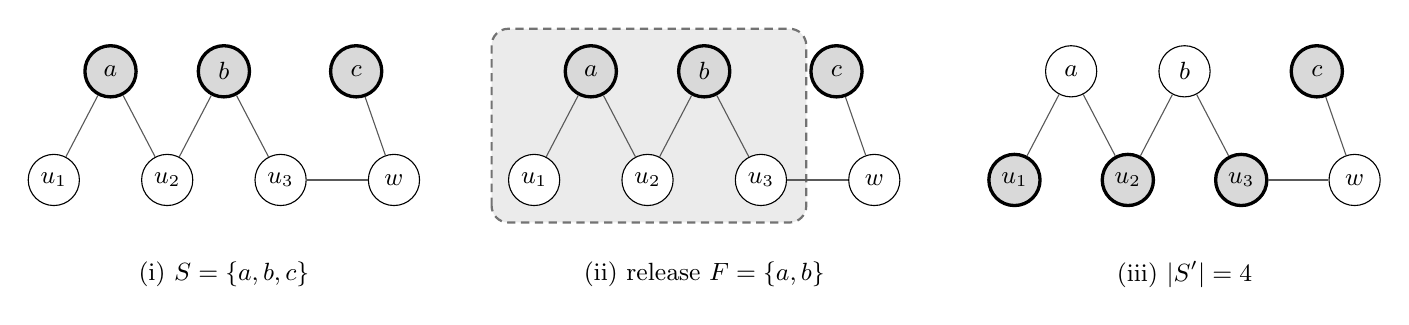
\begin{tikzpicture}[
  every node/.style={font=\small},
  vtx/.style={circle,draw,minimum size=6.5mm,inner sep=0pt,fill=white},
  ins/.style={vtx,fill=black!15,very thick},
  ed/.style={draw,black!65},
  x=12mm,y=12mm]

% ---- panel (i): the incumbent ----
\begin{scope}
  \node[ins] (a)  at (0,1.15)  {$a$};
  \node[ins] (b)  at (1.2,1.15){$b$};
  \node[ins] (c)  at (2.6,1.15){$c$};
  \node[vtx] (u1) at (-0.6,0) {$u_1$};
  \node[vtx] (u2) at (0.6,0)  {$u_2$};
  \node[vtx] (u3) at (1.8,0)  {$u_3$};
  \node[vtx] (w)  at (3.0,0)  {$w$};
  \foreach \s/\t in {a/u1,a/u2,b/u2,b/u3,c/w,u3/w} \draw[ed] (\s)--(\t);
  \node at (1.2,-1.0) {(i) $S=\{a,b,c\}$};
\end{scope}

% ---- panel (ii): the region ----
\begin{scope}[xshift=6.1cm]
  \node[ins] (a2)  at (0,1.15)  {$a$};
  \node[ins] (b2)  at (1.2,1.15){$b$};
  \node[ins] (c2)  at (2.6,1.15){$c$};
  \node[vtx] (u12) at (-0.6,0) {$u_1$};
  \node[vtx] (u22) at (0.6,0)  {$u_2$};
  \node[vtx] (u32) at (1.8,0)  {$u_3$};
  \node[vtx] (w2)  at (3.0,0)  {$w$};
  \begin{scope}[on background layer]
    \draw[rounded corners=6pt,fill=black!8,draw=black!55,thick,densely dashed]
      (-1.05,-0.45) rectangle (2.28,1.6);
  \end{scope}
  \foreach \s/\t in {a2/u12,a2/u22,b2/u22,b2/u32,c2/w2,u32/w2} \draw[ed] (\s)--(\t);
  \node at (1.2,-1.0) {(ii) release $F=\{a,b\}$};
\end{scope}

% ---- panel (iii): after the move ----
\begin{scope}[xshift=12.2cm]
  \node[vtx] (a3)  at (0,1.15)  {$a$};
  \node[vtx] (b3)  at (1.2,1.15){$b$};
  \node[ins] (c3)  at (2.6,1.15){$c$};
  \node[ins] (u13) at (-0.6,0) {$u_1$};
  \node[ins] (u23) at (0.6,0)  {$u_2$};
  \node[ins] (u33) at (1.8,0)  {$u_3$};
  \node[vtx] (w3)  at (3.0,0)  {$w$};
  \foreach \s/\t in {a3/u13,a3/u23,b3/u23,b3/u33,c3/w3,u33/w3} \draw[ed] (\s)--(\t);
  \node at (1.2,-1.0) {(iii) $|S'|=4$};
\end{scope}
\end{tikzpicture}
}
\caption{A region move that no swap-based neighbourhood expresses. Shaded
vertices are in the current solution. In (i) the incumbent $S=\{a,b,c\}$ is
maximal, so no vertex can simply be added. Releasing any \emph{single} vertex
also achieves nothing: $R(\{a\})=\{a,u_1\}$, $R(\{b\})=\{b,u_3\}$ and
$R(\{c\})=\{c,w\}$ each admit an independent set of size one, so every
$(1,k)$-swap returns the incumbent. Releasing $a$ and $b$ together gives the
region in (ii), $R(\{a,b\})=\{a,b,u_1,u_2,u_3\}$, because $u_2$ is the vertex
whose two incumbent neighbours are exactly $a$ and $b$. That region contains the
independent set $\{u_1,u_2,u_3\}$ of size three against the two vertices
released, and (iii) is the result: $|S'|=4$, which is $\alpha(G)$ here. Note that
$w$ stays outside the region --- its incumbent neighbour $c$ is not released ---
and that the edge $u_3w$ leaves the region. Theorem~\ref{thm:region}(a) forbids
edges from $R(F)$ to $S \setminus R(F)$ only, which is what makes the
substitution safe; edges to the rest of $V$ are unconstrained.}
\label{fig:region}
\end{figure}

The region is cheap to construct if the number of incumbent neighbours is
maintained.

\begin{proposition}[Cost of a move]
\label{prop:cost}
Let $t(u) = |N(u) \cap S|$ be maintained incrementally. Then $R(F)$ can be
constructed in time $O\!\left(\sum_{v \in F} \deg v\right)$, and the induced
subgraph $G[R(F)]$ in time $O\!\left(\sum_{v \in R(F)} \deg v\right)$.
\end{proposition}

\begin{proof}
Scanning the neighbourhoods of the vertices of $F$ and counting, for each
vertex $u$ outside $S$, how many of its neighbours lie in $F$, costs
$\sum_{v \in F} \deg v$. A vertex $u$ satisfies $N(u) \cap S \subseteq F$
exactly when that count equals $t(u)$, so membership in $R(F)$ is decided in
constant time per candidate, and only vertices adjacent to $F$ are candidates.
Maintaining $t$ costs $O(\deg v)$ whenever a vertex $v$ enters or leaves $S$,
which is charged to the move that changes it.
\end{proof}

The cost of the move is therefore dominated not by the size of the graph but by
the total degree of the region, and the exact sub-solve is performed on the
kernel of $G[R(F)]$ rather than on $G[R(F)]$ itself.

\begin{corollary}[Relation to classical swaps]
For $F = \{v\}$, $R(F) = \{v\} \cup \{u \notin S : N(u) \cap S = \{v\}\}$, which
is the set examined by a $(1,2)$-swap \cite{andrade2012}. Solving $G[R(F)]$
exactly therefore finds the best $(1,k)$-swap at $v$ for every $k$ at once, and
larger $F$ yields moves no swap-based neighbourhood expresses.
\end{corollary}

\section{Algorithm and implementation}
\label{sec:algorithm}

\subsection{The search}

Algorithm~\ref{alg:cascade} gives the overall structure. Kernelization runs
once; a \emph{dive} then constructs an initial solution by repeatedly discarding
a maximum-degree vertex and re-reducing, which reproduces reducing-peeling
\cite{chang2017}; the remaining budget goes to region moves.

\begin{algorithm}
\caption{\textsc{Cascade}}
\label{alg:cascade}
\begin{algorithmic}[1]
\State $(K,\mathit{trail}) \gets \textsc{Reduce}(G)$ \Comment{full rule set, bounded share of budget}
\While{$K \neq \emptyset$} \Comment{dive: cheap rules only}
  \State discard a maximum-degree vertex of $K$; re-reduce
\EndWhile
\State $S \gets \textsc{Maximalise}(\textsc{Lift}(\mathit{trail}))$
\State $W \gets$ kernel vertices and their neighbours \Comment{worklist of seeds}
\While{budget remains}
  \State $v \gets W.\textsc{pop}()$;\; $F \gets k$ incumbent vertices around $v$
  \State $R \gets F \cup \{u \notin S : N(u) \cap S \subseteq F\}$
  \State $T \gets \textsc{ExactMis}(G[R])$ \Comment{branch-and-reduce, bounded}
  \If{$|T| > |F|$} $S \gets (S \setminus R) \cup T$; push $R \cup N(R)$ onto $W$
  \ElsIf{$|T| = |F|$ \textbf{and} $T \neq F$ \textbf{and} on a plateau} $S \gets (S \setminus R) \cup T$
  \EndIf
  \State adapt $k$; occasionally perturb; restart if stuck
\EndWhile
\end{algorithmic}
\end{algorithm}

\paragraph{Where the search looks} Every vertex decided by a reduction belongs
to some maximum independent set, so an improving move must touch a vertex that
survived into the kernel. Seeding the sweep from the kernel and its neighbours
rather than from all of $V$ matters on graphs that reduce well: \texttt{com-lj}
has four million vertices and reduces to a kernel more than two orders of
magnitude smaller. The kernel size measured for every instance is in the run
records distributed with the source.

\paragraph{Choosing the neighbourhood size} The useful value of $k=|F|$ differs
by three orders of magnitude across instance families, so it is inferred rather
than set. A region that could not be solved to proven optimality within its
budget halves $k$; a run of regions solved to optimality without finding any
improvement doubles it. On meshes this settles at tens of released vertices; on
dense instances it settles at one or two, where the move degenerates to a
classical swap.

\paragraph{Escaping local optima} Because region moves never degrade the
incumbent, the search stalls at a solution that is optimal for every region of
the current size. Three mechanisms address this. \emph{Plateau moves} accept a
region optimum of equal size that differs from the incumbent, once a full sweep
has stopped producing gains; randomised tie-breaking in the sub-solver makes
repeated solves of the same region return different optima. \emph{Perturbation}
forces a vertex into the solution, evicts its blocking neighbours and lets
region moves repair the damage, with a change log that rolls back only the
touched vertices if the result is worse. \emph{Restarts} discard the incumbent
and dive again, keeping the best solution in an archive; the trigger is idle
time measured in multiples of the cost of one dive, since a restart must pay for
a re-dive. This keying matters: on the smallest instances the algorithm restarts
hundreds of times within a minute, while on the largest it never restarts.

\subsection{Data structures and throughput}
\label{sec:implementation}

Reductions and branching decisions both mutate the graph and must be reversible,
at every node of the sub-searches and after every region move. We use a compressed
adjacency array in which each entry stores the position of its twin, together
with a per-vertex pointer separating the live neighbours from the dead ones.
Deleting a vertex $v$ swaps its entry to the end of each live neighbour's range
and decrements that neighbour's pointer; undoing the deletion merely increments
the pointers again. Nothing has to be swapped back, because no later operation
touches an entry outside the live range. Both directions cost $O(\deg v)$ and
carry no payload, and degrees remain exact throughout.

Degree-2 folding introduces edges that do not fit in the static array; these go
into per-vertex overflow lists which are append-only and undone by a pop, and
which are allocated only for vertices that actually take part in a fold.

Two engineering details matter for throughput. First, each node of a sub-search
owns an exact list of its live vertices, built by filtering its parent's. An
earlier version shared one list and could drop a vertex when a fold created a new
one; the clique-cover bound then failed to cover that vertex, came out too small,
and pruned optimal solutions while still reporting that optimality had been
proven. Second, the sub-solver is reused across region moves instead of being
constructed afresh, since at a hundred thousand moves per minute the set-up of
the graph and reduction state costs more than the search itself.

To give these choices a number: on \texttt{del18}, 262\,144 vertices, the solver
kernelizes the whole graph in $1.16$\,s, completes its first dive $0.37$\,s
later, and then performs 107\,238 region moves in the remaining 58\,s, or one
every $543$\,$\mu$s. On \texttt{web-Stanford} the corresponding figures are
$0.69$\,s, $0.03$\,s and 96\,842 moves at $605$\,$\mu$s each. Those rates are
what the reuse of the sub-solver and the payload-free undo buy; the throughput,
not the asymptotics, is what makes an exactly-solved neighbourhood practical.

A third detail is worth reporting because its value is not obvious and grows
with scale. The reduction queue is seeded in increasing order of degree, so that
the cheap rules fire on the vertices most likely to trigger cascades before any
expensive test is attempted on a hub. Against the same solver seeding the queue
in plain vertex order, kernelization takes $0.84$\,s rather than $1.05$\,s on
\texttt{web-Stanford}, $4.87$ rather than $7.39$ on \texttt{as-skitter}, and
$13.98$ rather than $48.84$ on \texttt{com-lj}. The gain is a factor of $1.25$ at
282\,000 vertices and $3.5$ at four million: the ordering matters more the larger
the graph, because a rule applied in the wrong order does work that a later
deletion would have made unnecessary, and the number of such wasted applications
grows faster than the graph does. It is one line of counting sort.

The last of these details is the one that decides whether the solver keeps its
promise at all. Kernelization is run to exhaustion in principle, but on some
graphs exhaustion is unaffordable: on \texttt{soc-pokec}, 1.6 million vertices,
running the rules to a fixed point takes $180.5$\,s, three times the entire
60-second budget, so a solver that insisted on finishing would return nothing at
all. We therefore give kernelization a fixed share of the budget --- $0.3$ by
default --- and stop it where it stands when that share is spent, keeping
whatever reductions have been applied and continuing with the rest. On
\texttt{soc-pokec} the phase is cut off at $18.0$\,s, exactly the share, and the
solver returns 788\,868 within its budget. The truncation is recorded in the
run records, so a reader can see on which instances the kernel is partial.
This is the difference between a method that respects a deadline and one that
merely has a time limit in its interface.

Correctness is checked by comparing the exact solver against exhaustive search on
random graphs, repeating the comparison with each reduction rule disabled in
turn, and by verifying that every reported solution is independent and maximal.

\section{Computational study}
\label{sec:experiments}

\subsection{Setup}

All runs are performed on the same machine and are single-threaded: an Intel
Xeon at 2.10\,GHz with four cores and 15\,GB of memory, running Ubuntu 24.04,
with every solver compiled by GCC 13.3 at \texttt{-O3}. Every solver
receives the same wall-clock budget, measured around the entire process, so that
reading the instance and any construction phase are charged to the solver that
incurs them. This is deliberate: a solver whose construction phase cannot be
interrupted is genuinely less useful under a deadline, and
Table~\ref{tab:budget} reports how closely each solver keeps to the budget.

Every reported value is verified independently. A separate program re-reads the
original instance, confirms that the returned set contains no edge, and reports
its size; values that fail this check, or that a solver reports without emitting
the set itself, are not counted. This matters in practice: the reference
implementations of reducing-peeling print a size without the corresponding set,
so their numbers are marked unverified in the raw records.

Baselines are built from their authors' published sources, at the revision the
provisioning script pins, and with the authors' own build settings. ReduMIS and
OnlineMIS come from KaMIS \cite{lamm2017,dahlum2016}; reducing-peeling and the
near-linear kernelization from the implementation released with
Chang et al. \cite{chang2017}; NuMVC \cite{cai2013numvc} and FastVC
\cite{cai2017fastvc} from a library that carries the original implementations.
The last two solve the minimum vertex cover formulation, and we convert their
output to an independent set before verification. Each solver is given the
instance in the format its own implementation expects, converted by a single
tool distributed with our code, so that no solver pays a parsing penalty another
avoids.

The main tables carry no exact or integer-programming baseline. Those methods
answer a different question, and on most of this benchmark they do not answer it
within the budget; we report them separately in Section~\ref{sec:exact}, where
the comparison is on their own terms.

\subsection{Instances}

The benchmark comprises 27 instances in five families: Delaunay triangulations
and random geometric graphs, road networks, social networks, web graphs, and the
BHOSLIB \texttt{frb} collection generated from Model RB \cite{xu2007}. The first
family is generated with a fixed seed by a script included with the source; the
remainder are public.

One instance-preparation issue is worth recording, because it silently produces
wrong answers. The BHOSLIB instances are distributed in \emph{clique} form, and
the copies in common repositories are the dense clique graphs: \texttt{frb30-15-1}
there has 450 vertices and 83,198 edges. A maximum independent set of that file
has size 15, the domain size of the underlying construction, and every solver we
tested returns exactly 15 on it. The instance relevant to the present problem is
the complement, with 17,827 edges and independence number 30, and that is what
we use. Benchmarking the distributed file directly would have every solver agree
on a confidently wrong value.

\begin{table}[htbp]
\centering
\caption{Geometric (Delaunay and random geometric): size of the independent set found within the 60\,s budget (larger is better). Best value per instance in bold.}
\label{tab:quality-geometric}
\small
\begin{tabular}{lrrrrrr}
\toprule
Algorithm & \texttt{rgg16} & \texttt{del16} & \texttt{rgg18} & \texttt{del18} & \texttt{rgg20} & \texttt{del20} \\
\midrule
\textsc{Cascade} & \textbf{16086} & \textbf{20650} & \textbf{64278} & \textbf{82662} & \textbf{256994} & \textbf{330154} \\
ReduMIS & \textbf{16086} & 20640 & \textbf{64278} & 82385 & \textbf{256994} & 321566 \\
OnlineMIS & 16082 & 20634 & 63939 & 82031 & 242831 & 311006 \\
NearLinear & 16035 & 20284 & 64094 & 81211 & 256277 & 324619 \\
LinearTime & 15321 & 20213 & 61282 & 80881 & 244769 & 323438 \\
\bottomrule
\end{tabular}
\end{table}

\begin{table}[htbp]
\centering
\caption{Road networks: size of the independent set found within the 60\,s budget (larger is better). Best value per instance in bold.}
\label{tab:quality-road}
\small
\begin{tabular}{lrr}
\toprule
Algorithm & \texttt{roadNet-PA} & \texttt{roadNet-CA} \\
\midrule
\textsc{Cascade} & 533627 & \textbf{961851} \\
ReduMIS & \textbf{533628} & \textbf{961851} \\
OnlineMIS & 515876 & 924236 \\
NearLinear & 531184 & 957199 \\
LinearTime & 530910 & 956573 \\
\bottomrule
\end{tabular}
\end{table}

\begin{table}[htbp]
\centering
\caption{Social networks: size of the independent set found within the 60\,s budget (larger is better). Best value per instance in bold.}
\label{tab:quality-social}
\small
\begin{tabular}{lrrrrrrrrrr}
\toprule
Algorithm & \texttt{ca-AstroPh} & \texttt{ca-CondMat} & \texttt{email-Enron} & \texttt{com-dblp} & \texttt{com-amazon} & \texttt{com-youtube} & \texttt{soc-pokec-relationships} & \texttt{as-skitter} & \texttt{wiki-Talk} & \texttt{com-lj} \\
\midrule
\textsc{Cascade} & \textbf{6760} & \textbf{9612} & \textbf{22255} & \textbf{152131} & \textbf{174632} & \textbf{857945} & 788866 & 1170576 & \textbf{2338222} & \textbf{2085626} \\
ReduMIS & \textbf{6760} & \textbf{9612} & \textbf{22255} & \textbf{152131} & \textbf{174632} & \textbf{857945} & -- & \textbf{1170580} & \textbf{2338222} & \textbf{2085626} \\
OnlineMIS & \textbf{6760} & 9601 & 22227 & 152061 & 172685 & 857680 & 776663 & 1152300 & 2338207 & 2066610 \\
NearLinear & \textbf{6760} & \textbf{9612} & \textbf{22255} & \textbf{152131} & 174627 & \textbf{857945} & \textbf{789161} & 1170541 & \textbf{2338222} & 2085604 \\
LinearTime & 6759 & 9611 & \textbf{22255} & 152129 & 174612 & 857944 & 789003 & 1170410 & \textbf{2338222} & 2085353 \\
\bottomrule
\end{tabular}
\end{table}

\begin{table}[htbp]
\centering
\caption{Web graphs: size of the independent set found within the 60\,s budget (larger is better). Best value per instance in bold.}
\label{tab:quality-web}
\small
\begin{tabular}{lrr}
\toprule
Algorithm & \texttt{web-Stanford} & \texttt{web-BerkStan} \\
\midrule
\textsc{Cascade} & 163375 & 408380 \\
ReduMIS & \textbf{163390} & \textbf{408482} \\
OnlineMIS & 162453 & 406062 \\
NearLinear & 163198 & 408054 \\
LinearTime & 163121 & 407716 \\
\bottomrule
\end{tabular}
\end{table}

\begin{table}[htbp]
\centering
\caption{BHOSLIB \texttt{frb}: size of the independent set found within the 60\,s budget (larger is better). Best value per instance in bold.}
\label{tab:quality-bhoslib}
\small
\begin{tabular}{lrrrrrrr}
\toprule
Algorithm & \texttt{frb30-15-1} & \texttt{frb35-17-1} & \texttt{frb40-19-1} & \texttt{frb45-21-1} & \texttt{frb50-23-1} & \texttt{frb53-24-1} & \texttt{frb59-26-1} \\
\midrule
\textsc{Cascade} & \textbf{30} & 34 & \textbf{40} & \textbf{43} & 48 & 50 & 56 \\
ReduMIS & \textbf{30} & \textbf{35} & \textbf{40} & \textbf{43} & \textbf{49} & \textbf{51} & \textbf{57} \\
OnlineMIS & 29 & 33 & 39 & 42 & 48 & 49 & 56 \\
NearLinear & 24 & 27 & 27 & 33 & 35 & 38 & 43 \\
LinearTime & 22 & 25 & 29 & 32 & 33 & 40 & 43 \\
\bottomrule
\end{tabular}
\end{table}

\begin{table}[htbp]
\centering
\caption{Aggregate over all 27 instances. The gap of an algorithm on an instance is $(\text{best found by any algorithm} - \text{its value}) / \text{best found by any algorithm}$.}
\label{tab:aggregate}
\fittable{
\begin{tabular}{lrrrr}
\toprule
Algorithm & \#best & \#solved & mean gap & max gap \\
\midrule
\textsc{Cascade} & 17 & 27 & 0.414\% & 2.857\% \\
ReduMIS & 23 & 26 & 0.113\% & 2.575\% \\
OnlineMIS & 1 & 27 & 1.791\% & 5.732\% \\
NearLinear & 7 & 27 & 6.831\% & 32.500\% \\
LinearTime & 2 & 27 & 7.742\% & 32.653\% \\
\bottomrule
\end{tabular}
}
\end{table}

\begin{table}[htbp]
\centering
\caption{Paired Wilcoxon signed-rank test of \textsc{Cascade} against each baseline over the instances both solved, at the 60\,s budget. A verdict names the better solver when $p<0.05$.}
\label{tab:wilcoxon}
\fittable{
\begin{tabular}{lrrrrrr}
\toprule
Baseline & pairs & win & tie & loss & $p$ & verdict \\
\midrule
ReduMIS & 26 & 3 & 14 & 9 & 0.1951 & -- \\
FastVC & 27 & 13 & 8 & 6 & 0.0300 & \textsc{Cascade} \\
NearLinear & 27 & 20 & 6 & 1 & 0.0001 & \textsc{Cascade} \\
NuMVC & 26 & 18 & 2 & 6 & 0.0008 & \textsc{Cascade} \\
OnlineMIS & 27 & 23 & 4 & 0 & $<10^{-4}$ & \textsc{Cascade} \\
LinearTime & 27 & 24 & 2 & 1 & $<10^{-4}$ & \textsc{Cascade} \\
\bottomrule
\end{tabular}
}
\end{table}

\begin{table}[htbp]
\centering
\caption{Wall-clock time actually taken under a 60\,s budget, over all instances. Time is measured around the whole process, so it includes reading and any construction phase.}
\label{tab:budget}
\begin{tabular}{lrrrr}
\toprule
Algorithm & median & mean & max & runs $>1.5\times$ budget \\
\midrule
\textsc{Cascade} & 60.1 & 48.3 & 75.0 & 0 \\
ReduMIS & 60.2 & 69.7 & 660.2 & 2 \\
OnlineMIS & 60.0 & 44.0 & 66.8 & 0 \\
NearLinear & 0.2 & 1.1 & 15.4 & 0 \\
LinearTime & 0.1 & 0.3 & 2.5 & 0 \\
\bottomrule
\end{tabular}
\end{table}

\begin{table}[htbp]
\centering
\caption{Ablation: each row disables one component. Values in brackets are the change from the full algorithm.}
\label{tab:ablation}
\small
\begin{tabular}{lrrrrrrr}
\toprule
Configuration & \texttt{del16} & \texttt{del18} & \texttt{rgg16} & \texttt{roadNet-PA} & \texttt{web-Stanford} & \texttt{frb40-19-1} & \texttt{frb59-26-1} \\
\midrule
full & 20648 & 82661 & 16086 & 533627 & 163375 & 40 & 56 \\
no region moves & 20369 (-279) & 81639 (-1022) & 16085 (-1) & 533385 (-242) & 163369 (-6) & 27 (-13) & 42 (-14) \\
no perturbation/restarts & 20656 (+8) & 82657 (-4) & 16086 (+0) & 533627 (+0) & 163375 (+0) & 38 (-2) & 56 (+0) \\
no LP reduction & 20652 (+4) & 82666 (+5) & 16086 (+0) & 533627 (+0) & 163373 (-2) & 40 (+0) & 57 (+1) \\
decision-space moves & 20383 (-265) & 81639 (-1022) & 16086 (+0) & 533385 (-242) & 163369 (-6) & 34 (-6) & 49 (-7) \\
\bottomrule
\end{tabular}
\end{table}


\subsection{Solution quality}

Tables~\ref{tab:quality-geometric}--\ref{tab:quality-bhoslib} give the size of
the independent set each solver returned, by family.

On the geometric family \textsc{Cascade} attains the best value of the seven
solvers on every instance. On the three Delaunay instances it is strictly ahead
of all of them, and the margin grows with size: $+7$ on \texttt{del16}, $+77$ on
\texttt{del18} and $+264$ on \texttt{del20}, measured against the strongest
baseline on each, which is ReduMIS on the first and FastVC on the other two.
Read against ReduMIS alone the same three margins are $+7$, $+271$ and $+8500$,
because ReduMIS degrades sharply at the largest size while FastVC does not; this
is why we report the comparison against the per-instance best rather than
against a single reference solver. The $+8500$ should also be read with
Section~\ref{sec:longbudget}, which shows that it shrinks to $+1550$ when both
solvers are given ten times the budget: on \texttt{del20} ReduMIS converges
slowly rather than to a worse answer. The margin over the strongest baseline,
by contrast, is unaffected by the budget. In relative terms the margin over the
strongest baseline is small in every case --- $0.03\%$, $0.09\%$ and $0.08\%$ ---
but it is consistent, and it is the only family in which any solver separates
itself from the rest. This is also the family whose kernels remain a large
fraction of the input, so it is where the choice of what to do after
kernelization matters most, and where a move that restructures tens of vertices
at once has the most to work with. On the random geometric graphs the reduction
rules are far more effective, and \textsc{Cascade} and ReduMIS reach the same
value on all three sizes; for \texttt{rgg16} and \texttt{rgg18} the exact
solvers of Section~\ref{sec:exact} prove that this common value is optimal, so
no solver could have done better there.

On road networks and on most social networks the strong solvers agree to within
a handful of vertices, because the kernels are a small fraction of the input:
\texttt{com-lj} has four million vertices and near-linear kernelization leaves
9780 of them. What separates the solvers there is robustness rather than
quality, and the differences that remain run in both directions. \textsc{Cascade}
ties ReduMIS exactly on \texttt{com-lj} and is four vertices behind it on
\texttt{as-skitter} out of $1.17$ million; on \texttt{soc-pokec} it is $0.06\%$
behind FastVC, the best value there. Robustness is where the gap is visible:
ReduMIS returned nothing on \texttt{soc-pokec} within eleven minutes, and NuMVC
returned nothing on \texttt{com-lj} within sixteen, while \textsc{Cascade}
produced a verified solution on every instance in the benchmark.

On web graphs \textsc{Cascade} is behind ReduMIS by 15 and 102 vertices, which
is $0.009\%$ and $0.025\%$. On the BHOSLIB family it is the weaker tool. It
reaches the known optimum of \texttt{frb30-15-1}, as do ReduMIS, NuMVC and
FastVC, but on the other six instances it is one or two vertices short of the
best value, and that best value is NuMVC's or FastVC's on every one of them ---
45 against our 43 on \texttt{frb45-21-1}, 58 against our 56 on
\texttt{frb59-26-1}. Because these optima are small, a two-vertex shortfall is a
$4.4\%$ relative gap, the largest we record anywhere. The structural
reason is given in Section~\ref{sec:move}: on a dense graph almost every vertex
outside the incumbent has several incumbent neighbours, so releasing a small
$F$ unlocks nothing while releasing a large one makes the region the whole
graph. The move degenerates, and specialised local search is the better tool.

\begin{figure}[htbp]
\centering
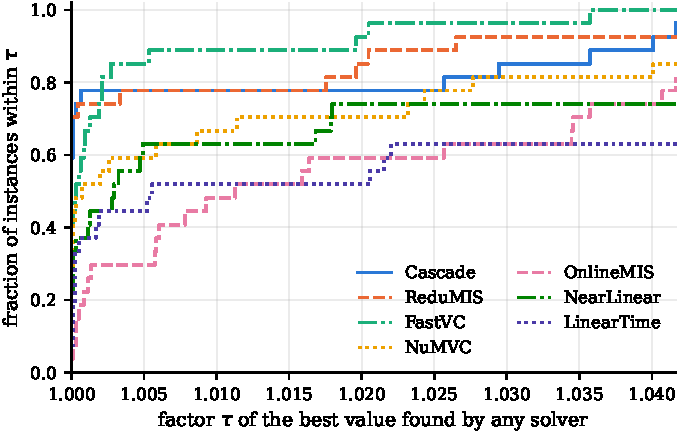
\includegraphics[width=0.78\textwidth]{figures/profile}
\caption{Performance profile on solution quality. For each instance the ratio is
the best value any solver found divided by the value this solver returned, so
$\tau = 1$ means it matched the best. The axis is truncated to keep the region
where the curves separate legible: an arrow marks a curve that continues beyond
it, which here is reducing-peeling and near-linear kernelization, whose worst
ratios are $1.52$ and $1.48$. Below $1.0$ at the right-hand edge without an
arrow means a run that returned no solution at all, namely ReduMIS on
\texttt{soc-pokec} and NuMVC on \texttt{com-lj}. Note that the profile is a
\emph{relative} measure and therefore weights the small dense instances heavily,
where losing a single vertex is already a $2$--$3\%$ ratio;
Table~\ref{tab:aggregate} and the absolute margins below give the complementary
view.}
\label{fig:profile}
\end{figure}

\begin{table}[htbp]
\centering
\caption{Where the advantage over \textsc{ReduMIS} comes from, per instance family, at the 60-second budget. \emph{Net} is the sum over the family of $|S_{\textsc{cascade}}|-|S_{\textsc{ReduMIS}}|$; higher is better. The one instance on which \textsc{ReduMIS} returned nothing within the budget is excluded from its family's counts.}
\label{tab:whence}
\begin{tabular}{l r r r r r}
\toprule
Family & Instances & Ahead & Tied & Behind & Net \\
\midrule
geometric & 6 & 3 & 3 & 0 & +8778 \\
road & 2 & 0 & 1 & 1 & -1 \\
web & 2 & 0 & 0 & 2 & -117 \\
social $^{*}$ & 10 & 0 & 8 & 1 & -4 \\
bhoslib & 7 & 0 & 2 & 5 & -5 \\
\midrule
\textbf{All} & 27 & 3 & 14 & 9 & +8651 \\
\bottomrule
\end{tabular}
\\[2pt]\footnotesize $^{*}$ one instance excluded: \textsc{ReduMIS} exceeded the budget.
\end{table}


\subsection{Aggregate comparison}

Counting wins is misleading here, because instances differ in scale by four
orders of magnitude and a one-vertex loss on a 450-vertex instance is not
comparable to a five-thousand-vertex win on a million-vertex one. We therefore
report both the mean relative gap (Table~\ref{tab:aggregate}) and a paired
Wilcoxon signed-rank test (Table~\ref{tab:wilcoxon}).

The test finds \textsc{Cascade} significantly better than five of the six
baselines, including both solvers from the vertex cover local search line, and
finds no significant difference against ReduMIS ($p = 0.195$). The comparison
against ReduMIS deserves to be unpacked, because a single aggregate hides its
shape. Table~\ref{tab:whence} decomposes it by family. Over the 26 instances
both solved, \textsc{Cascade} is ahead on three and behind on nine, and ties on
the remaining fourteen; summed over all of them it is ahead by 8778 vertices and
behind by 127, for a net of $+8651$. Nearly all of that net comes from one
instance, \texttt{del20}, and the deficit is concentrated in the two web graphs.
The honest reading is not that \textsc{Cascade} dominates ReduMIS but that the
two are equal on most of this benchmark, that \textsc{Cascade} degrades far more
gracefully on the largest geometric instance, and that ReduMIS holds a small
edge on web graphs. That is exactly what a non-significant $p$-value over
twenty-six paired observations should be taken to mean.

Figure~\ref{fig:profile} shows the same data as a performance profile.
\textsc{Cascade} matches the best value on 16 of the 27 instances, reaches
within $0.07\%$ of it on a further five, and returns a solution on every
instance, which ReduMIS and NuMVC do not. Its curve is then flat from
$\tau \approx 1.0006$ to $\tau \approx 1.026$, and the six instances beyond that
break are the whole of the rest of the BHOSLIB family. The break is an artefact
of scale rather than of behaviour: a one-vertex shortfall on a 35-vertex optimum
is a $2.9\%$ ratio, and a two-vertex shortfall on a 45-vertex optimum is
$4.7\%$, so instances whose absolute loss is one or two vertices sit further to
the right than instances whose absolute loss is a hundred. This is the
complementary weakness of the profile to the one noted for the absolute margins,
and the two views should be read together.

Table~\ref{tab:budget} should be read alongside these results. NuMVC checks its
cutoff only between search steps, so under a 60\,s budget it takes 204\,s on
average and exceeds 90\,s on twelve of the 27 instances; it is therefore
compared here under conditions that favour it, and is still behind.

\subsection{Seed study}

The solvers compared here are randomised, so we repeated a subset of ten
instances with five seeds each. Table~\ref{tab:seeds} reports the best and mean
size, and Figure~\ref{fig:seeds} the spread.

The single-seed picture holds. On best-of-five, \textsc{Cascade} is
significantly ahead of FastVC ($p = 0.016$), NuMVC ($p = 0.023$) and OnlineMIS
($p = 0.008$), and indistinguishable from ReduMIS ($p = 0.81$); on the mean the
verdicts are the same, with \textsc{Cascade} ahead of OnlineMIS on all ten
instances.

The figure also shows a limitation. On every geometric, road and web instance
our solver's five runs collapse to a line: the spread is at most $0.024\%$, and
on two instances all five seeds return the same value. On the BHOSLIB instances
it widens by two orders of magnitude, to $2.5\%$ on \texttt{frb40-19-1} and
$2.0\%$ on \texttt{frb53-24-1}. It is not the most variable solver there ---
OnlineMIS spreads $5.1\%$ and $3.9\%$ on those two instances --- but it is
markedly less stable than ReduMIS and FastVC, which return the same value on
every seed of both, and on \texttt{frb40-19-1} that value is 40 against our 39
or 40. This is the same degeneracy discussed in
Section~\ref{sec:move} seen from another angle: when the region move cannot
find traction, what remains is the restart mechanism, and outcomes then depend
on which restart happens to land well. A practitioner running a single seed on a
dense instance should expect variance that the other families do not show.

\begin{table}[htbp]
\centering
\caption{Five seeds per instance at the 60\,s budget: best and mean size found. The spread is negligible on every family except BHOSLIB.}
\label{tab:seeds}
\small
\fittable{
\begin{tabular}{lrrrrr}
\toprule
Instance & \textsc{Cascade} & ReduMIS & FastVC & NuMVC & OnlineMIS \\
\midrule
\texttt{del16} & \textbf{20647 / 20644.2} & 20641 / 20639.4 & 20642 / 20637.0 & 20192 / 20178.2 & 20634 / 20631.6 \\
\texttt{del18} & \textbf{82656 / 82652.2} & 82393 / 82369.0 & 82589 / 82581.0 & 80727 / 80699.2 & 82042 / 82030.8 \\
\texttt{del20} & \textbf{330125 / 330104.2} & 321935 / 321503.0 & 329833 / 329818.2 & 311469 / 311427.0 & 311198 / 311117.6 \\
\texttt{frb40-19-1} & \textbf{40 / 39.6} & \textbf{40 / 40.0} & \textbf{40 / 40.0} & \textbf{40 / 39.8} & 39 / 38.4 \\
\texttt{frb53-24-1} & 51 / 50.4 & 51 / 51.0 & 51 / 51.0 & \textbf{52 / 52.0} & 51 / 50.0 \\
\texttt{frb59-26-1} & 56 / 56.0 & 57 / 57.0 & 57 / 56.6 & \textbf{58 / 58.0} & 56 / 55.8 \\
\texttt{rgg18} & \textbf{64278 / 64278.0} & \textbf{64278 / 64278.0} & 64255 / 64252.4 & 62550 / 62532.6 & 63911 / 63907.4 \\
\texttt{roadNet-PA} & \textbf{533628 / 533627.2} & \textbf{533628 / 533627.2} & 532575 / 532560.4 & 513102 / 513084.4 & 515949 / 515874.2 \\
\texttt{web-BerkStan} & 408402 / 408389.4 & \textbf{408482 / 408482.0} & 406338 / 406292.6 & 404996 / 404978.6 & 406051 / 405951.4 \\
\texttt{web-Stanford} & 163375 / 163373.0 & \textbf{163390 / 163390.0} & 162972 / 162964.8 & 162480 / 162461.6 & 162450 / 162433.8 \\
\bottomrule
\end{tabular}
}
\end{table}


\begin{figure}[htbp]
\centering
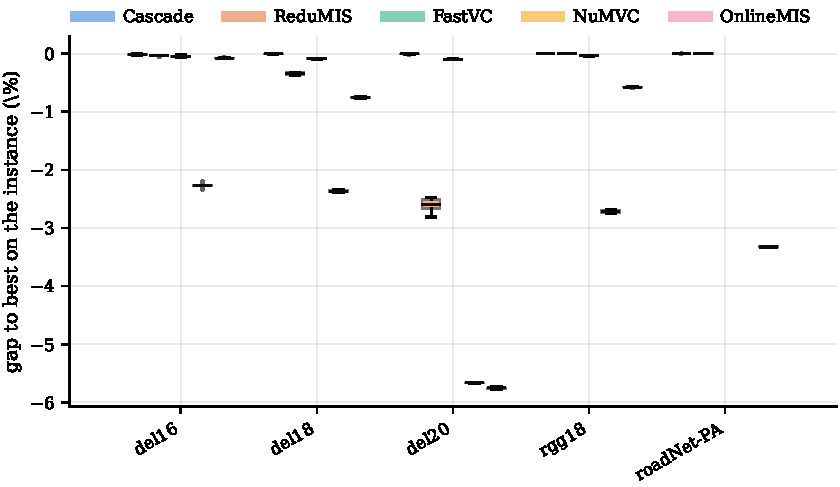
\includegraphics[width=\textwidth]{figures/seeds}
\caption{Spread over five seeds, as a percentage of the best value reached on
each instance. Boxes show the quartiles and the median; whiskers the range.}
\label{fig:seeds}
\end{figure}

\subsection{Convergence}
\label{sec:convergence}

Table~\ref{tab:longbudget} shows what each solver reaches by the end of its
budget; Figure~\ref{fig:convergence} shows how it gets there. Four instances
were re-run with every improvement of the incumbent recorded against the wall
clock. Only the three solvers that report improvements as they happen are
plotted; the reduction-only baselines produce a single point.

The shapes differ more than the endpoints do. On \texttt{del18} and
\texttt{roadNet-PA} our solver reaches a value the others need most of the
budget to approach, and then flattens: the kernelization and the first dive do
most of the work, and the region moves refine it. On \texttt{web-Stanford} it
converges almost immediately and improves six times in sixty seconds, which is
the same observation the long-budget run makes from the other direction --- there
is very little left to find once the graph has been reduced. The dense instance
inverts the picture. All three solvers finish on the same value of 40, but NuMVC
reaches it after $0.2$ seconds and FastVC after $0.8$, where we need $6.6$: on a
graph this dense the region move has to work its way to what a specialised local
search finds almost at once, and the tie at the deadline hides a large
difference in how quickly it was reached.

\begin{figure}[htbp]
\centering
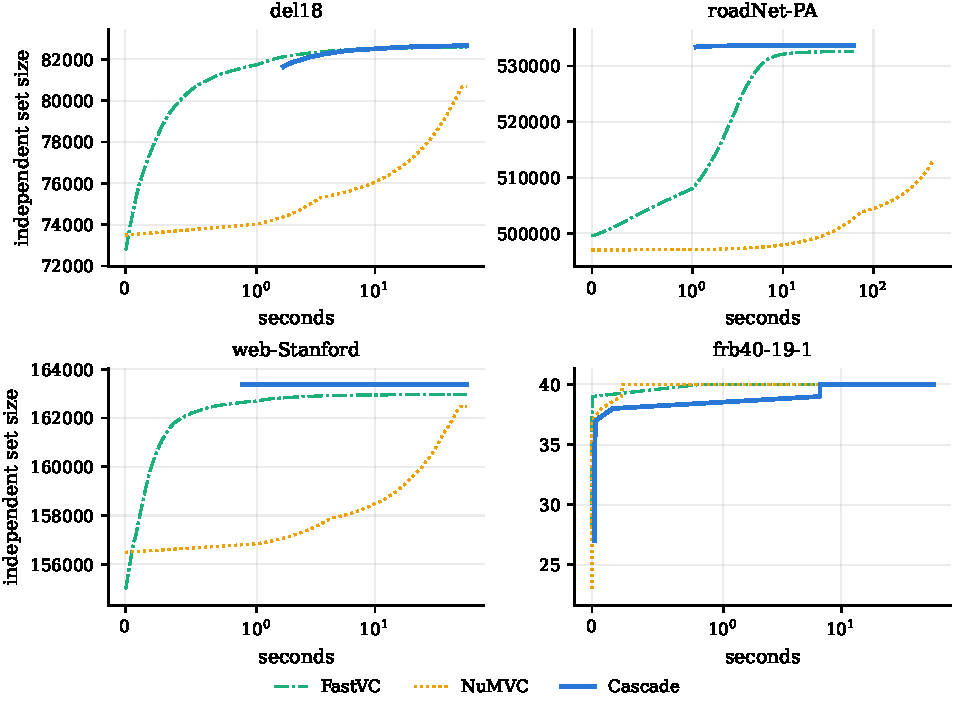
\includegraphics[width=\textwidth]{figures/convergence}
\caption{Incumbent size against wall-clock time at a 60-second budget, on a
symmetric-log time axis so the first second is legible. Note that the solvers
report at different granularities: ours records one point per search batch
(between 6 and 586 points here) while NuMVC and FastVC report every individual
improvement (up to 33\,000), so the apparent smoothness of a curve reflects how
often a solver reports, not how often it improves.}
\label{fig:convergence}
\end{figure}

\subsection{The long budget}
\label{sec:longbudget}

The main study gives every solver 60 seconds. That choice needs defending,
because a budget short enough to favour one convergence profile over another
would decide the comparison by itself. We therefore repeated four instances,
one per family, at ten times the budget. Table~\ref{tab:longbudget} gives the
result, and the comparison that matters is with the 60-second tables.

On three of the four instances the extra budget buys almost nothing.
\textsc{Cascade} and ReduMIS return \emph{exactly} the same value on
\texttt{roadNet-CA} and on \texttt{web-BerkStan} at 600 seconds as at 60, and on
\texttt{frb59-26-1} every solver moves by at most a single vertex. Those
instances are converged well inside the shorter budget, and nothing in the main
tables is an artefact of stopping early.

\texttt{del20} is the exception, and it qualifies our own headline. At 60
seconds \textsc{Cascade} leads ReduMIS there by 8500 vertices; at 600 seconds it
leads by 1550. ReduMIS gains 7417 vertices from the extra time and NuMVC 6227,
against 467 for \textsc{Cascade} and 390 for FastVC. The large gap to ReduMIS
that Section~\ref{sec:experiments} reports on the largest Delaunay instance is
therefore substantially a statement about convergence rate rather than about
final quality: ReduMIS gets to a similar place, it simply takes an order of
magnitude longer to do it.

Two things survive that correction. \textsc{Cascade} still returns the best value
on \texttt{del20} at the long budget, 330\,533 against FastVC's 330\,192, and its
margin over the \emph{strongest} baseline is essentially unchanged by the extra
time --- 264 vertices at 60 seconds, 341 at 600. The advantage that the paper
claims over the best available alternative is robust to the budget. What is not
robust, and what we therefore do not claim, is the much larger gap to ReduMIS
specifically.

The table also shows the other side of the same coin, and it is not in our
favour. ReduMIS reaches its final value on \texttt{web-BerkStan} in 67 seconds
and on \texttt{roadNet-CA} in 69, matching or beating what \textsc{Cascade}
returns after ten times as long. On graphs whose kernel reduces to a small
fraction of the input, a solver that finishes kernelization and stops is simply
the better tool, and no amount of neighbourhood search recovers the difference.
This is the same boundary that Section~\ref{sec:move} predicts from the
structure of the move, seen from the direction of running time rather than
solution quality.

\begin{table}[htbp]
\centering
\small
\caption{Solution size and wall-clock seconds at a 600-second budget, ten times the budget of the main study. HIGHER IS BETTER for size, lower for time; \textbf{bold} marks the best size on an instance. The comparison of interest is with Table~\ref{tab:quality-geometric} and its companions, measured at 60 seconds: outside the dense instance, the extra budget changes almost nothing.}
\label{tab:longbudget}
\begin{tabular}{l r@{\,/\,}l r@{\,/\,}l r@{\,/\,}l r@{\,/\,}l}
\toprule
Solver & \multicolumn{2}{c}{\texttt{del20}} & \multicolumn{2}{c}{\texttt{roadNet-CA}} & \multicolumn{2}{c}{\texttt{web-BerkStan}} & \multicolumn{2}{c}{\texttt{frb59-26-1}} \\
& size & s & size & s & size & s & size & s \\
\midrule
\textsc{Cascade} & \textbf{330533} & 601 & \textbf{961851} & 603 & 408380 & 602 & \multicolumn{2}{c}{---} \\
ReduMIS & 328983 & 602 & \textbf{961851} & 69 & \textbf{408482} & 67 & 57 & 328 \\
NuMVC & 317648 & 671 & 915773 & 1003 & 406663 & 650 & \textbf{59} & 600 \\
FastVC & 330192 & 604 & 960024 & 601 & \multicolumn{2}{c}{---} & 57 & 600 \\
\bottomrule
\end{tabular}
\end{table}


\subsection{Parameter sensitivity}
\label{sec:sensitivity}

The method exposes several tunable parameters, and a reader is entitled to ask
whether the results depend on having found good values for them.
Table~\ref{tab:sensitivity} varies four of them one at a time over a wide range,
holding the rest at their defaults, on three instances from different families.
The comparison that makes the numbers interpretable is with the seed-to-seed
spread of Section~\ref{sec:experiments}: a parameter whose whole range moves the
answer by less than the noise between two seeds is not a parameter the user has
to think about.

On the two large sparse instances that is what happens. Over ranges spanning a
factor of seven to sixteen, \texttt{kernel\_share}, \texttt{lns\_start\_free}
and \texttt{lns\_slice} move the result by at most $0.013\%$ on \texttt{del18}
and $0.001\%$ on \texttt{web-Stanford}, against a seed spread of $0.024\%$ on
that family. On \texttt{web-Stanford} two of them are exactly flat: every value of
\texttt{kernel\_share} from $0.1$ to $0.7$, and every value of
\texttt{lns\_slice} from $0.01$ to $0.2$, returns the same 163\,375.

One parameter is genuinely sensitive, and we report it as such.
\texttt{restart\_idle\_dives} moves \texttt{del18} by $0.081\%$, three times the
seed spread, and the shape is informative: 82\,592 at 50, 82\,639 at 100, 82\,659
at the default 200, then 82\,655 at both 400 and 800. Restarting too eagerly
costs real quality, while restarting too lazily costs almost nothing. The
default sits at the top of that curve rather than on its slope, but a reader
porting this method to a new family should know that this is the one dial worth
checking, and that the safe direction to err in is upwards.

The dense instance is where this design runs out of resolution, and we say so
rather than reading meaning into it. The spreads there are $2.5\%$ to $5\%$, but
every value in the block is 38, 39 or 40, and the seed study already reports a
$2.5\%$ spread on this family from seed alone. A single run per setting cannot
separate a parameter effect from that noise. What can be said is bounded: no
setting we tried collapses performance, and \texttt{lns\_start\_free}$=8$ returns
40 where the default returns 39 --- which is either a better setting or a luckier
seed, and this experiment cannot tell which.

\begin{table}[htbp]
\centering
\small
\caption{Parameter sensitivity. Each block varies one parameter over its range with the others held at their defaults; $\star$ marks the default. Cells are the size returned at a 60-second budget, HIGHER IS BETTER. The \emph{spread} line under each block is $100\,(\max-\min)/\max$ over that block, per instance, to be read against the seed-to-seed spread of Section~\ref{sec:experiments}: $0.024\%$ on the geometric family and up to $2.5\%$ on BHOSLIB.}
\label{tab:sensitivity}
\fittable{
\begin{tabular}{l r r r r }
\toprule
Parameter & Value & \texttt{del18} & \texttt{frb40-19-1} & \texttt{web-Stanford} \\
\midrule
\texttt{kernel\_share} & 0.1 & 82656 & 39 & 163375 \\
 & 0.2 & 82655 & 39 & 163375 \\
 & 0.3$\star$ & 82655 & 40 & 163375 \\
 & 0.5 & 82656 & 40 & 163375 \\
 & 0.7 & 82655 & 39 & 163375 \\
\cmidrule(lr){3-5}
& \emph{spread \%} & \emph{0.001} & \emph{2.500} & \emph{0.000} \\\\
\midrule
\texttt{lns\_start\_free} & 1 & 82648 & 39 & 163374 \\
 & 2 & 82650 & 39 & 163375 \\
 & 4$\star$ & 82655 & 39 & 163375 \\
 & 8 & 82650 & 40 & 163376 \\
 & 16 & 82659 & 38 & 163374 \\
\cmidrule(lr){3-5}
& \emph{spread \%} & \emph{0.013} & \emph{5.000} & \emph{0.001} \\\\
\midrule
\texttt{lns\_slice} & 0.01 & 82651 & 39 & 163375 \\
 & 0.02 & 82649 & 40 & 163375 \\
 & 0.05$\star$ & 82656 & 39 & 163375 \\
 & 0.1 & 82656 & 39 & 163375 \\
 & 0.2 & 82656 & 39 & 163375 \\
\cmidrule(lr){3-5}
& \emph{spread \%} & \emph{0.008} & \emph{2.500} & \emph{0.000} \\\\
\midrule
\texttt{restart\_idle\_dives} & 50 & 82592 & 39 & 163373 \\
 & 100 & 82639 & 39 & 163375 \\
 & 200$\star$ & 82659 & 40 & 163375 \\
 & 400 & 82655 & 39 & 163375 \\
 & 800 & 82655 & 40 & 163375 \\
\cmidrule(lr){3-5}
& \emph{spread \%} & \emph{0.081} & \emph{2.500} & \emph{0.001} \\\\
\bottomrule
\end{tabular}
}
\end{table}


\subsection{Exact solvers}
\label{sec:exact}

The method proposed here is a heuristic, and the question of how far its answers
sit from optimal is separate from how they compare with other heuristics. To
place them we ran three exact solvers and one integer-programming solver on the
instances small enough to admit them: the branch-and-reduce solver built from
our own components (\textsc{Cascade}-exact, the sub-solver of
Section~\ref{sec:implementation} applied to the whole graph), VCSolver
\cite{akiba2016}, the winner of the vertex cover track of PACE 2019
\cite{pace2019,hespe2020}, and HiGHS on the natural
integer program. Table~\ref{tab:exact} reports the results.

Three conclusions follow, and only the first is favourable to us. On the
instances that reduce almost completely --- \texttt{ca-AstroPh},
\texttt{ca-CondMat}, \texttt{email-Enron} --- all four prove optimality, and our
sub-solver is the fastest of them --- by a factor of 25 to 40 over HiGHS, three
to five over VCSolver, and a more modest 1.1 to 1.4 over the PACE portfolio ---
which is the property
the region move depends on: the sub-problems it generates are of exactly this
shape, and at some 1800 moves per second they must each be solved in a fraction
of a millisecond.

Second, our exact solver is not competitive as an exact solver. On the BHOSLIB
family the PACE 2019 portfolio proves the optimum of \texttt{frb30-15-1},
\texttt{frb35-17-1} and \texttt{frb40-19-1} in under four seconds each, while
ours returns 25, 28 and 30 against the true 30, 35 and 40 and proves nothing.
It is built to be restarted millions of times on graphs of a few dozen vertices,
not to prove optimality on a dense graph of a thousand, and the table shows the
cost of that choice. Where a proof is wanted on instances of this kind, the
portfolio approach is the right tool.

Third, the integer-programming route is not a usable baseline at this scale, and
we record its failures rather than omitting it. HiGHS matches the optimum on the
three easy instances but exceeds the 60-second budget on most others, taking up
to 360\,s; on \texttt{frb45-21-1} through \texttt{frb53-24-1} it returns a single
vertex, on \texttt{rgg18} none at all, and on \texttt{del18} and
\texttt{web-Stanford} it emits no solution we could verify. On
\texttt{email-Enron} it reports optimality but the solution it writes has 22\,253
vertices against the 22\,255 that the other three solvers prove optimal and that
our verifier confirms; we therefore treat its optimality claims as unreliable
and its numbers as a lower bound on what a tuned commercial solver would do.
This is a statement about the formulation at this size, not about HiGHS: the
natural model has one variable per vertex and one constraint per edge, which for
the larger instances in the benchmark means tens of millions of constraints.

\begin{table}[htbp]
\centering
\small
\caption{Exact and integer-programming solvers under a 60-second budget, on the instances where any of them terminates. Each pair of columns gives the size returned and the wall-clock seconds; \textbf{bold} marks a value the solver proved optimal, and \textit{t/o} that it returned no solution within the budget. Higher is better for size, lower for time.}
\label{tab:exact}
\fittable{
\begin{tabular}{l l r r r r r r r r }
\toprule
& & \multicolumn{2}{c}{\textsc{Cascade}-exact} & \multicolumn{2}{c}{VCSolver} & \multicolumn{2}{c}{PACE 2019} & \multicolumn{2}{c}{HiGHS} \\
\cmidrule(lr){3-4}\cmidrule(lr){5-6}\cmidrule(lr){7-8}\cmidrule(lr){9-10}
Instance & Family & size & s & size & s & size & s & size & s \\
\midrule
\texttt{ca-AstroPh} & social & \textbf{6760} & 0.1 & \textbf{6760} & 0.3 & \textbf{6760} & 0.1 & \textbf{6760} & 4.0 \\
\texttt{ca-CondMat} & social & \textbf{9612} & 0.0 & \textbf{9612} & 0.2 & \textbf{9612} & 0.1 & \textbf{9612} & 1.3 \\
\texttt{email-Enron} & social & \textbf{22255} & 0.1 & \textbf{22255} & 0.4 & \textbf{22255} & 0.1 & \textbf{22253} & 2.0 \\
\texttt{del16} & geometric & 20474 & 60.1 & \textit{---} & \textit{t/o} & \textit{---} & \textit{t/o} & 9679 & 60.5 \\
\texttt{del18} & geometric & 73928 & 83.2 & \textit{---} & \textit{t/o} & \textit{---} & \textit{t/o} & \textit{---} & \textit{t/o} \\
\texttt{rgg16} & geometric & 16086 & 60.1 & \textbf{16086} & 0.7 & \textbf{16086} & 0.4 & 16086 & 60.6 \\
\texttt{rgg18} & geometric & 64271 & 60.3 & \textbf{64278} & 2.3 & \textbf{64278} & 2.2 & 0 & 240.8 \\
\texttt{web-Stanford} & web & 163376 & 60.6 & \textit{---} & \textit{t/o} & \textit{---} & \textit{t/o} & \textit{---} & \textit{t/o} \\
\texttt{frb30-15-1} & bhoslib & 25 & 60.0 & \textit{---} & \textit{t/o} & \textbf{30} & 1.8 & 28 & 60.1 \\
\texttt{frb35-17-1} & bhoslib & 28 & 60.0 & \textit{---} & \textit{t/o} & \textbf{35} & 2.5 & 30 & 60.2 \\
\texttt{frb40-19-1} & bhoslib & 30 & 60.0 & \textit{---} & \textit{t/o} & \textbf{40} & 3.6 & 2 & 60.2 \\
\texttt{frb45-21-1} & bhoslib & 34 & 60.1 & \textit{---} & \textit{t/o} & \textit{---} & \textit{t/o} & 1 & 60.2 \\
\texttt{frb50-23-1} & bhoslib & 35 & 60.1 & \textit{---} & \textit{t/o} & \textit{---} & \textit{t/o} & 1 & 60.2 \\
\texttt{frb53-24-1} & bhoslib & 37 & 60.0 & \textit{---} & \textit{t/o} & \textit{---} & \textit{t/o} & 1 & 60.8 \\
\texttt{frb59-26-1} & bhoslib & 42 & 60.1 & \textit{---} & \textit{t/o} & \textit{---} & \textit{t/o} & 30 & 60.3 \\
\bottomrule
\end{tabular}
}
\end{table}


\subsection{Ablation}
\label{sec:ablation}

Table~\ref{tab:ablation} reports four variants on seven instances spanning the
families: \textsc{no-lns} disables region moves entirely, leaving kernelization
plus the greedy dive and its restarts; \textsc{dive} replaces the region move
with the decision-space move described in Section~\ref{sec:move}; \textsc{no-pert}
removes the perturbation step; and \textsc{no-lp} removes the
Nemhauser--Trotter LP reduction. These are separate runs from the main study, so
the full-solver column differs from Table~\ref{tab:quality-geometric} by a few
vertices; the comparison is within the table.

The region move is the component that carries the result. Removing it costs
$1.2\%$ on \texttt{del18} and $1.4\%$ on \texttt{del16} --- an order of magnitude
more than the margin the full solver holds over the strongest baseline on those
instances --- and $32.5\%$ on \texttt{frb40-19-1}, where the fallback is reduced
to a restarting greedy. Summed over the seven instances the loss is 1577
vertices. Nothing else in the solver comes close to that.

The other three results are negative, and we report them as such. The
decision-space move recovers almost none of the gap: on \texttt{del18},
\texttt{roadNet-PA} and \texttt{web-Stanford} it returns exactly the value
obtained with no neighbourhood move at all (81\,639, 533\,385 and 163\,369), so
on those instances it contributes nothing whatever. It is the move we designed
first, and the ablation is what showed it to be worthless; only on the dense
instances does it recover part of the loss. It survives in the implementation
as an option, not as a default.

Perturbation and the LP reduction are both within noise on this benchmark.
Removing perturbation changes the summed total by $+2$ vertices, and hurts only
\texttt{frb40-19-1}, by two. Removing the LP reduction changes it by $+8$, and
on \texttt{frb59-26-1} the solver without it returns 57 rather than 56 --- which
is the value ReduMIS reaches and we do not. We keep both because each is cheap
and each is standard, and because a seven-instance ablation is too small to
conclude that they never help; but we have no evidence from these runs that
either pays for itself, and a reader looking to reimplement the method should
start with the region move and add the rest only if measurement justifies it.

\subsection{Replication on different hardware}
\label{sec:replication}

A computational study is only as convincing as its independence from the machine
it was run on. We therefore repeated the comparison on a second, unrelated
platform: virtual machines with two Intel Xeon cores at 2.20\,GHz and 12\,GB of
memory, against the four-core workstation used for the main tables. Every solver
was rebuilt from source on that platform by the provisioning script included
with our code, so nothing is carried over except the source.

Two properties of the replication are worth stating explicitly. First, all
solvers for a given instance were run on the same virtual machine, so each row
of the replication table is internally consistent; only different rows may come
from different machines, and those machines are of identical specification.
Splitting a single instance's solvers across machines would have made the
comparison meaningless, since the budget is a wall-clock budget and the amount
of work that fits into it depends on the processor. Second, the two largest
instances were excluded, because 12\,GB of memory is not enough for them; the
replication therefore covers 25 of the 27 instances.

Table~\ref{tab:replication} reports the outcome. The question a reader needs
answered is whether the \emph{ranking} in the main tables is a property of the
solvers or of the machine, and on that the answer is unambiguous: on all 25
instances, the set of solvers attaining the best value on the replication
machine intersects the set attaining it on the original machine. No solver
changes place with another. A reader can therefore take the comparisons in
Section~\ref{sec:experiments} as being about the algorithms.

The individual values move a little, and the table shows where. The two
deterministic solvers, reducing-peeling and near-linear kernelization, return
\emph{identical} values on all 25 instances, which is the control: it confirms that
the instances, the conversions and the verifier are the same on both platforms,
so any difference elsewhere comes from the solver rather than from the pipeline.
The five randomised solvers differ by a fraction of a percent on average, and
what difference there is concentrates on BHOSLIB, where the optima are small
enough that a one-vertex change is one to two percent. Away from that family our
own solver returns the same value on both machines on every road, web and social
instance, and differs by an average of $0.016\%$ on the geometric family.

Two caveats belong with this. The replication machine is slower, so a solver
that spends its whole budget does less work within it; that is visible as the
larger spreads for the vertex cover local search solvers, which have no
reduction phase to fall back on, and most sharply as NuMVC exceeding the cutoff
altogether on \texttt{roadNet-CA}, an instance it completed on the faster
machine. And a fixed wall-clock budget on two machines
of different speed is not the same experiment twice --- it is the same
\emph{protocol} twice, which is what a practitioner choosing a solver under a
deadline actually faces.

\begin{table}[htbp]
\centering
\small
\caption{Replication on a second platform. Each cell is the mean, over the instances of that family, of $100\,|s_2-s_1|/s_1$ where $s_1$ is the size the solver returned on the machine used for the main tables and $s_2$ the size it returned on the replication machine. LOWER IS BETTER: zero means the solver returned the same value on both machines. \emph{Same} counts the instances on which it did so exactly, out of 24.}
\label{tab:replication}
\begin{tabular}{l r r r r r r r}
\toprule
Solver & Geometric & Road & Web & Social & Bhoslib & Same & Max \\
\midrule
\textsc{Cascade} & 0.016 & 0.000 & 0.000 & 0.000 & 0.366 & 18/24 & 2.56 \\
ReduMIS & 0.124 & 0.000 & 0.000 & 0.000 & 0.000 & 22/24 & 0.74 \\
OnlineMIS & 0.608 & 0.164 & 0.157 & 0.000 & 0.000 & 16/24 & 1.76 \\
NuMVC & 0.021 & 0.006 & 0.008 & 0.002 & 0.560 & 8/24 & 2.00 \\
FastVC & 0.058 & 0.019 & 0.009 & 0.000 & 1.144 & 9/24 & 2.22 \\
NearLinear & 0.000 & 0.000 & 0.000 & 0.000 & 0.000 & 24/24 & 0.00 \\
LinearTime & 0.000 & 0.000 & 0.000 & 0.000 & 0.000 & 24/24 & 0.00 \\
\bottomrule
\end{tabular}
\end{table}


\subsection{Threats to validity}
\label{sec:threats}

\paragraph{Measurement} All timings are wall-clock and include reading the
instance. Kernelization is bounded by a share of the budget but is not
interruptible in the middle of a rule, so our own solver can overrun slightly;
Table~\ref{tab:budget} reports the distribution for every solver, and the
baseline that overruns most is the one our comparison is least favourable to.

\paragraph{Unverified values} The reference implementations of reducing-peeling
report a solution size without emitting the corresponding set, so those values
cannot be checked by our verifier and are taken on trust. All other values in
this paper were re-derived from an emitted solution.

\paragraph{Instance provenance} The Delaunay and random geometric instances are
generated rather than taken from an archive. They are reproducible from the seed
in the generator we distribute, but they are not byte-identical to the instances
of the same name used in earlier papers, so cross-paper comparison of absolute
values on those families is not meaningful; comparisons within this paper are
unaffected because every solver sees the same files.

\paragraph{Randomisation} Our solver, ReduMIS, OnlineMIS, NuMVC and FastVC are
randomised. The main table reports a single seed per instance; the seed study
repeats a subset with five seeds and reports both the best and the mean, and the
statistical test is computed on per-instance aggregates.

\paragraph{Failures} Two solvers failed to return any solution on some
instance within the cutoff, which we report as a failure rather than excluding
the instance. Excluding them would have removed exactly the cases that
distinguish the solvers.

\paragraph{Implementation maturity} The baselines are mature codebases. NuMVC
and FastVC have been refined by their authors and others since 2013 and 2015
respectively, and the KaMIS solvers likewise; ours is a research implementation
written for this paper. A comparison of wall-clock results under a fixed budget
cannot separate the merit of an algorithm from the quality of the code that runs
it, and the reader should not read our numbers as though it could.

We nevertheless report the comparison as measured, for three reasons. The
strongest baseline on this benchmark, ReduMIS, is as heavily engineered as the
vertex cover solvers, and it is the one against which we claim the least: no
test in this paper separates us from it. Excluding the mature implementations
would remove exactly the solvers a practitioner would otherwise choose. And the
bias runs against us where we win and for us where we lose, which is the less
convenient direction: our margins over NuMVC on the large sparse instances ---
46\,054 vertices on \texttt{roadNet-CA}, 18\,645 on \texttt{del20} --- would only
be larger if implementation quality were equalised, while our one- and two-vertex
deficits on BHOSLIB might narrow.

We do not, therefore, attribute the BHOSLIB result to implementation maturity.
Section~\ref{sec:move} gives a structural reason for it --- on a dense graph the
region is either empty or the whole graph, so the move degenerates --- and the
convergence traces support that reading: NuMVC reaches the final value there in
$0.2$ seconds, which is not the signature of a better-tuned inner loop but of a
search whose neighbourhood suits the instance.

\paragraph{Build differences between the two platforms} The replication
machines rebuilt the solver from source, and that source had by then acquired
the tracing used for Figure~\ref{fig:convergence}, which the machine used for
the main tables did not carry. The two builds are therefore not bit-identical,
and the replication in Section~\ref{sec:replication} varies build as well as
machine. We measured the size of that confound rather than assuming it away:
running both builds on the same machine, with the same seed and budget, they
return identical values on \texttt{del18}, \texttt{rgg16}, \texttt{web-Stanford}
and \texttt{roadNet-PA}, and differ by five vertices out of 20\,647 on
\texttt{del16}, which is $0.024\%$. That is the same order as the seed-to-seed
spread we report for the geometric family, and an order of magnitude below any
difference the replication is used to argue about. It does not affect the
ranking, which is what that section claims; but the per-instance agreement
counts in Table~\ref{tab:replication} should be read as bounded by it rather
than as pure machine effects.

\paragraph{How narrow the positive result is} This is the threat we consider
most serious, and the reader should weigh it against the aggregate tests. Our
solver is strictly ahead of every baseline on three of 27 instances. They are
the three Delaunay graphs, they form one family, and they were generated by us.
On thirteen instances it merely ties the best value, and on eleven it is behind.
The Wilcoxon tests in Table~\ref{tab:wilcoxon} are computed over relative gaps,
and the gaps that make them significant are largely the ones where NuMVC,
OnlineMIS and the peeling solvers degrade on large sparse graphs rather than
ones where our solver pulls ahead; against the one baseline that does not
degrade there, ReduMIS, no test in this paper finds a significant difference.
The defensible claim is therefore narrow: the region move gives a consistent
advantage on graphs whose kernel stays large, it costs nothing on graphs that
reduce away, and it is the wrong tool on dense graphs. A benchmark containing
more large-kernel families would test that claim better than this one does, and
we do not know of a public collection of them.

\section{Conclusions}
\label{sec:conclusions}

We introduced a neighbourhood for the maximum independent set problem that is
solved exactly rather than sampled, and showed that it is separated from the rest
of the incumbent and therefore monotone. Data reductions, normally applied once
as preprocessing, are what make the move affordable, and the ablation confirms
that the move is where the improvement comes from: removing it costs more than
the entire margin over the baselines.

Two limitations are worth stating plainly. On dense instances the region either
stays empty or grows to the whole graph, so the move degenerates and specialised
local search remains preferable. On web graphs the method is slightly behind the
strongest baseline, and we have not identified a structural reason for this.

The region definition and Theorem~\ref{thm:region} carry over verbatim to the
weighted problem by replacing cardinality with weight, which is the natural next
step given that recent activity in this area has concentrated on the weighted
case.

\section*{Data availability}
Source code, instance generators and the raw per-run records are available at
\url{https://github.com/vinhqdang/max_independence_set}.

\appendix

\section{Instance provenance}
\label{app:provenance}

Table~\ref{tab:provenance} records where each instance came from, so that the
benchmark set can be rebuilt exactly. Three points deserve emphasis, because each
is a way in which two studies can report different numbers for what they believe
is the same graph.

First, the real-world instances are distributed as directed or multiply-listed
edge lists. We read every file as undirected, discard self-loops and duplicate
edges, and renumber the vertices consecutively; the $n$ and $m$ in the table are
the values after this normalisation, and they are what our solver and every
baseline receive. Isolated vertices are retained rather than dropped, since
dropping them would inflate the reported independence number relative to studies
that keep them.

Second, the BHOSLIB instances are published in two forms, and the distinction is
easy to miss. The Network Repository archive ships the \emph{clique} form, whose
independence number is the size of a Model-RB domain rather than the advertised
$\alpha$: on \texttt{frb30-15-1} that form has 83\,198 edges and every solver we
tried returned exactly 15. The form used here, and the one the published
$\alpha$ values refer to, is its complement, with 17\,827 edges and $\alpha=30$.
Our converter takes the complement explicitly. A study that omits this step is
not solving a hard instance at all, and its BHOSLIB numbers cannot be compared
with anyone else's.

Third, the geometric instances are generated rather than downloaded. They come
from \texttt{tools/gen\_instances.py} at seed 1: the Delaunay instances are the
Delaunay triangulation of $2^{k}$ uniform points in the unit square, and the
random geometric instances connect points within the radius that gives an
expected average degree of 8. The generator is deterministic given the seed, so
the instances in the table are reproducible, but they are \emph{not} the DIMACS
implementation-challenge graphs of the same names, and the two should not be
compared.

\footnotesize
\setlength{\tabcolsep}{3pt}
\begin{longtable}{l l r r r r l}
\caption{Provenance and basic statistics of the 27 benchmark instances. $\bar{d}$ is the average degree and $\Delta$ the maximum degree. Sources: SNAP is \texttt{snap.stanford.edu/data}, where each instance is the file of its own name; $^{\dagger}$ Network Repository \texttt{bhoslib}, used in complement as Section~\ref{sec:experiments} explains; $^{\ddagger}$ produced by \texttt{tools/gen\_instances.py} at seed 1.}\label{tab:provenance}\\
\toprule
Instance & Family & $n$ & $m$ & $\bar{d}$ & $\Delta$ & Source \\
\midrule
\endfirsthead
\multicolumn{7}{l}{\itshape Table~\ref{tab:provenance}, continued}\\
\toprule
Instance & Family & $n$ & $m$ & $\bar{d}$ & $\Delta$ & Source \\
\midrule
\endhead
\midrule \multicolumn{7}{r}{\itshape continued on next page}\\
\endfoot
\bottomrule
\endlastfoot
\texttt{rgg16} & geometric & 65,501 & 260,438 & 8.0 & 24 & generated$^{\ddagger}$ \\
\texttt{del16} & geometric & 65,536 & 196,583 & 6.0 & 20 & generated$^{\ddagger}$ \\
\texttt{rgg18} & geometric & 262,011 & 1,046,301 & 8.0 & 23 & generated$^{\ddagger}$ \\
\texttt{del18} & geometric & 262,144 & 786,401 & 6.0 & 21 & generated$^{\ddagger}$ \\
\texttt{rgg20} & geometric & 1,048,171 & 4,188,702 & 8.0 & 24 & generated$^{\ddagger}$ \\
\texttt{del20} & geometric & 1,048,576 & 3,145,692 & 6.0 & 22 & generated$^{\ddagger}$ \\
\texttt{roadNet-PA} & road & 1,088,092 & 1,541,898 & 2.8 & 9 & SNAP \\
\texttt{roadNet-CA} & road & 1,965,206 & 2,766,607 & 2.8 & 12 & SNAP \\
\texttt{web-Stanford} & web & 281,903 & 1,992,636 & 14.1 & 38,625 & SNAP \\
\texttt{web-BerkStan} & web & 685,230 & 6,649,470 & 19.4 & 84,230 & SNAP \\
\texttt{ca-AstroPh} & social & 18,772 & 198,050 & 21.1 & 504 & SNAP \\
\texttt{ca-CondMat} & social & 23,133 & 93,439 & 8.1 & 279 & SNAP \\
\texttt{email-Enron} & social & 36,692 & 183,831 & 10.0 & 1,383 & SNAP \\
\texttt{com-dblp} & social & 317,080 & 1,049,866 & 6.6 & 343 & SNAP \\
\texttt{com-amazon} & social & 334,863 & 925,872 & 5.5 & 549 & SNAP \\
\texttt{com-youtube} & social & 1,134,890 & 2,987,624 & 5.3 & 28,754 & SNAP \\
\texttt{soc-pokec-relationships} & social & 1,632,803 & 22,301,964 & 27.3 & 14,854 & generated$^{\ddagger}$ \\
\texttt{as-skitter} & social & 1,696,415 & 11,095,298 & 13.1 & 35,455 & SNAP \\
\texttt{wiki-Talk} & social & 2,394,385 & 4,659,565 & 3.9 & 100,029 & SNAP \\
\texttt{com-lj} & social & 3,997,962 & 34,681,189 & 17.3 & 14,815 & generated$^{\ddagger}$ \\
\texttt{frb30-15-1} & bhoslib & 450 & 17,827 & 79.2 & 122 & NetRep$^{\dagger}$ \\
\texttt{frb35-17-1} & bhoslib & 595 & 27,856 & 93.6 & 132 & NetRep$^{\dagger}$ \\
\texttt{frb40-19-1} & bhoslib & 760 & 41,314 & 108.7 & 178 & NetRep$^{\dagger}$ \\
\texttt{frb45-21-1} & bhoslib & 945 & 59,186 & 125.3 & 188 & NetRep$^{\dagger}$ \\
\texttt{frb50-23-1} & bhoslib & 1,150 & 80,072 & 139.3 & 208 & NetRep$^{\dagger}$ \\
\texttt{frb53-24-1} & bhoslib & 1,272 & 94,227 & 148.2 & 232 & NetRep$^{\dagger}$ \\
\texttt{frb59-26-1} & bhoslib & 1,534 & 126,555 & 165.0 & 277 & NetRep$^{\dagger}$ \\
\end{longtable}
\setlength{\tabcolsep}{6pt}
\normalsize


\section{Complete per-instance results}
\label{app:full}

Table~\ref{tab:appendix} lists every run behind the summary tables, so that the
aggregates can be checked against the individual measurements. The raw records,
including the seed study and the replication, are distributed with the source.

\begin{longtable}{llrr rr}
\caption{Complete per-instance results at the 60\,s budget: size found and wall-clock seconds. A dash means the solver returned no solution within the cutoff.}\label{tab:appendix}\\
\toprule
Instance & Solver & $n$ & $m$ & size & seconds \\
\midrule
\endfirsthead
\toprule Instance & Solver & $n$ & $m$ & size & seconds \\ \midrule \endhead
\bottomrule \endfoot
\texttt{rgg16} & \textsc{Cascade} & 65,501 & 260,438 & 16086 & 60.1 \\
 & ReduMIS &  &  & 16086 & 9.5 \\
 & OnlineMIS &  &  & 16082 & 60.1 \\
 & NuMVC &  &  & 15905 & 60.3 \\
 & FastVC &  &  & 16085 & 60.0 \\
 & NearLinear &  &  & 16035 & 0.1 \\
 & LinearTime &  &  & 15321 & 0.0 \\
\addlinespace
\texttt{del16} & \textsc{Cascade} & 65,536 & 196,583 & 20647 & 60.1 \\
 & ReduMIS &  &  & 20640 & 60.2 \\
 & OnlineMIS &  &  & 20630 & 60.1 \\
 & NuMVC &  &  & 20180 & 60.3 \\
 & FastVC &  &  & 20638 & 60.0 \\
 & NearLinear &  &  & 20284 & 0.1 \\
 & LinearTime &  &  & 20213 & 0.0 \\
\addlinespace
\texttt{rgg18} & \textsc{Cascade} & 262,011 & 1,046,301 & 64278 & 60.3 \\
 & ReduMIS &  &  & 64278 & 12.6 \\
 & OnlineMIS &  &  & 63912 & 60.5 \\
 & NuMVC &  &  & 62548 & 87.2 \\
 & FastVC &  &  & 64242 & 60.2 \\
 & NearLinear &  &  & 64094 & 0.3 \\
 & LinearTime &  &  & 61282 & 0.1 \\
\addlinespace
\texttt{del18} & \textsc{Cascade} & 262,144 & 786,401 & 82656 & 60.2 \\
 & ReduMIS &  &  & 82385 & 60.7 \\
 & OnlineMIS &  &  & 82019 & 60.4 \\
 & NuMVC &  &  & 80695 & 120.7 \\
 & FastVC &  &  & 82579 & 60.1 \\
 & NearLinear &  &  & 81211 & 0.7 \\
 & LinearTime &  &  & 80881 & 0.1 \\
\addlinespace
\texttt{rgg20} & \textsc{Cascade} & 1,048,171 & 4,188,702 & 256994 & 61.3 \\
 & ReduMIS &  &  & 256994 & 23.4 \\
 & OnlineMIS &  &  & 242366 & 61.7 \\
 & NuMVC &  &  & 239118 & 490.2 \\
 & FastVC &  &  & 256680 & 60.8 \\
 & NearLinear &  &  & 256277 & 1.8 \\
 & LinearTime &  &  & 244769 & 0.5 \\
\addlinespace
\texttt{del20} & \textsc{Cascade} & 1,048,576 & 3,145,692 & 330066 & 61.1 \\
 & ReduMIS &  &  & 321566 & 258.2 \\
 & OnlineMIS &  &  & 311146 & 61.7 \\
 & NuMVC &  &  & 311421 & 428.9 \\
 & FastVC &  &  & 329802 & 60.6 \\
 & NearLinear &  &  & 324619 & 4.7 \\
 & LinearTime &  &  & 323438 & 0.4 \\
\addlinespace
\texttt{roadNet-PA} & \textsc{Cascade} & 1,088,092 & 1,541,898 & 533627 & 60.8 \\
 & ReduMIS &  &  & 533628 & 37.2 \\
 & OnlineMIS &  &  & 515876 & 61.2 \\
 & NuMVC &  &  & 513067 & 451.1 \\
 & FastVC &  &  & 532571 & 60.3 \\
 & NearLinear &  &  & 531184 & 0.6 \\
 & LinearTime &  &  & 530910 & 0.1 \\
\addlinespace
\texttt{roadNet-CA} & \textsc{Cascade} & 1,965,206 & 2,766,607 & 961851 & 61.5 \\
 & ReduMIS &  &  & 961851 & 62.1 \\
 & OnlineMIS &  &  & 924236 & 62.2 \\
 & NuMVC &  &  & 915797 & 911.9 \\
 & FastVC &  &  & 959909 & 60.6 \\
 & NearLinear &  &  & 957199 & 1.8 \\
 & LinearTime &  &  & 956573 & 0.3 \\
\addlinespace
\texttt{ca-AstroPh} & \textsc{Cascade} & 18,772 & 198,050 & 6760 & 0.1 \\
 & ReduMIS &  &  & 6760 & 0.2 \\
 & OnlineMIS &  &  & 6760 & 60.1 \\
 & NuMVC &  &  & 6760 & 61.3 \\
 & FastVC &  &  & 6760 & 60.0 \\
 & NearLinear &  &  & 6760 & 0.0 \\
 & LinearTime &  &  & 6759 & 0.0 \\
\addlinespace
\texttt{ca-CondMat} & \textsc{Cascade} & 23,133 & 93,439 & 9612 & 0.1 \\
 & ReduMIS &  &  & 9612 & 0.1 \\
 & OnlineMIS &  &  & 9601 & 0.0 \\
 & NuMVC &  &  & 9611 & 60.5 \\
 & FastVC &  &  & 9612 & 60.0 \\
 & NearLinear &  &  & 9612 & 0.0 \\
 & LinearTime &  &  & 9611 & 0.0 \\
\addlinespace
\texttt{email-Enron} & \textsc{Cascade} & 36,692 & 183,831 & 22255 & 0.1 \\
 & ReduMIS &  &  & 22255 & 0.2 \\
 & OnlineMIS &  &  & 22227 & 0.1 \\
 & NuMVC &  &  & 22253 & 60.2 \\
 & FastVC &  &  & 22255 & 60.0 \\
 & NearLinear &  &  & 22255 & 0.0 \\
 & LinearTime &  &  & 22255 & 0.0 \\
\addlinespace
\texttt{com-dblp} & \textsc{Cascade} & 317,080 & 1,049,866 & 152131 & 0.4 \\
 & ReduMIS &  &  & 152131 & 0.6 \\
 & OnlineMIS &  &  & 152061 & 0.6 \\
 & NuMVC &  &  & 152112 & 85.9 \\
 & FastVC &  &  & 152131 & 60.2 \\
 & NearLinear &  &  & 152131 & 0.1 \\
 & LinearTime &  &  & 152129 & 0.1 \\
\addlinespace
\texttt{com-amazon} & \textsc{Cascade} & 334,863 & 925,872 & 174632 & 60.3 \\
 & ReduMIS &  &  & 174632 & 10.1 \\
 & OnlineMIS &  &  & 172685 & 0.6 \\
 & NuMVC &  &  & 174510 & 114.1 \\
 & FastVC &  &  & 174605 & 60.2 \\
 & NearLinear &  &  & 174627 & 0.1 \\
 & LinearTime &  &  & 174612 & 0.1 \\
\addlinespace
\texttt{com-youtube} & \textsc{Cascade} & 1,134,890 & 2,987,624 & 857945 & 1.3 \\
 & ReduMIS &  &  & 857945 & 1.8 \\
 & OnlineMIS &  &  & 857680 & 1.7 \\
 & NuMVC &  &  & 857708 & 143.2 \\
 & FastVC &  &  & 857945 & 60.6 \\
 & NearLinear &  &  & 857945 & 0.2 \\
 & LinearTime &  &  & 857944 & 0.2 \\
\addlinespace
\texttt{soc-pokec-relationships} & \textsc{Cascade} & 1,632,803 & 22,301,964 & 788866 & 72.9 \\
 & ReduMIS &  &  & -- & 660.2 \\
 & OnlineMIS &  &  & 776663 & 66.8 \\
 & NuMVC &  &  & 787320 & 444.4 \\
 & FastVC &  &  & 789352 & 64.0 \\
 & NearLinear &  &  & 789161 & 15.4 \\
 & LinearTime &  &  & 789003 & 1.6 \\
\addlinespace
\texttt{as-skitter} & \textsc{Cascade} & 1,696,415 & 11,095,298 & 1170576 & 64.5 \\
 & ReduMIS &  &  & 1170580 & 64.7 \\
 & OnlineMIS &  &  & 1152300 & 6.3 \\
 & NuMVC &  &  & 1168352 & 266.2 \\
 & FastVC &  &  & 1168417 & 61.9 \\
 & NearLinear &  &  & 1170541 & 0.7 \\
 & LinearTime &  &  & 1170410 & 0.5 \\
\addlinespace
\texttt{wiki-Talk} & \textsc{Cascade} & 2,394,385 & 4,659,565 & 2338222 & 2.5 \\
 & ReduMIS &  &  & 2338222 & 34.0 \\
 & OnlineMIS &  &  & 2338207 & 3.1 \\
 & NuMVC &  &  & 2338220 & 66.0 \\
 & FastVC &  &  & 2338222 & 61.1 \\
 & NearLinear &  &  & 2338222 & 0.3 \\
 & LinearTime &  &  & 2338222 & 0.3 \\
\addlinespace
\texttt{com-lj} & \textsc{Cascade} & 3,997,962 & 34,681,189 & 2085626 & 75.0 \\
 & ReduMIS &  &  & 2085626 & 68.8 \\
 & OnlineMIS &  &  & 2066610 & 16.9 \\
 & NuMVC &  &  & -- & 960.0 \\
 & FastVC &  &  & 2085169 & 67.5 \\
 & NearLinear &  &  & 2085604 & 2.2 \\
 & LinearTime &  &  & 2085353 & 2.5 \\
\addlinespace
\texttt{web-Stanford} & \textsc{Cascade} & 281,903 & 1,992,636 & 163375 & 60.7 \\
 & ReduMIS &  &  & 163390 & 31.3 \\
 & OnlineMIS &  &  & 162453 & 60.7 \\
 & NuMVC &  &  & 162453 & 92.3 \\
 & FastVC &  &  & 162953 & 60.3 \\
 & NearLinear &  &  & 163198 & 0.3 \\
 & LinearTime &  &  & 163121 & 0.1 \\
\addlinespace
\texttt{web-BerkStan} & \textsc{Cascade} & 685,230 & 6,649,470 & 408380 & 61.7 \\
 & ReduMIS &  &  & 408482 & 59.8 \\
 & OnlineMIS &  &  & 406062 & 61.9 \\
 & NuMVC &  &  & 405003 & 131.2 \\
 & FastVC &  &  & 406323 & 60.9 \\
 & NearLinear &  &  & 408054 & 0.7 \\
 & LinearTime &  &  & 407716 & 0.2 \\
\addlinespace
\texttt{frb30-15-1} & \textsc{Cascade} & 450 & 17,827 & 30 & 60.0 \\
 & ReduMIS &  &  & 30 & 60.4 \\
 & OnlineMIS &  &  & 29 & 60.0 \\
 & NuMVC &  &  & 30 & 60.0 \\
 & FastVC &  &  & 30 & 60.0 \\
 & NearLinear &  &  & 24 & 0.0 \\
 & LinearTime &  &  & 22 & 0.0 \\
\addlinespace
\texttt{frb35-17-1} & \textsc{Cascade} & 595 & 27,856 & 34 & 60.0 \\
 & ReduMIS &  &  & 35 & 60.5 \\
 & OnlineMIS &  &  & 33 & 60.0 \\
 & NuMVC &  &  & 35 & 60.0 \\
 & FastVC &  &  & 35 & 60.0 \\
 & NearLinear &  &  & 27 & 0.0 \\
 & LinearTime &  &  & 25 & 0.0 \\
\addlinespace
\texttt{frb40-19-1} & \textsc{Cascade} & 760 & 41,314 & 39 & 60.0 \\
 & ReduMIS &  &  & 40 & 61.2 \\
 & OnlineMIS &  &  & 39 & 60.0 \\
 & NuMVC &  &  & 40 & 60.0 \\
 & FastVC &  &  & 40 & 60.0 \\
 & NearLinear &  &  & 27 & 0.1 \\
 & LinearTime &  &  & 29 & 0.0 \\
\addlinespace
\texttt{frb45-21-1} & \textsc{Cascade} & 945 & 59,186 & 43 & 60.0 \\
 & ReduMIS &  &  & 43 & 60.6 \\
 & OnlineMIS &  &  & 42 & 60.0 \\
 & NuMVC &  &  & 45 & 60.1 \\
 & FastVC &  &  & 45 & 60.0 \\
 & NearLinear &  &  & 33 & 0.1 \\
 & LinearTime &  &  & 32 & 0.0 \\
\addlinespace
\texttt{frb50-23-1} & \textsc{Cascade} & 1,150 & 80,072 & 48 & 60.0 \\
 & ReduMIS &  &  & 49 & 61.1 \\
 & OnlineMIS &  &  & 48 & 60.0 \\
 & NuMVC &  &  & 50 & 60.1 \\
 & FastVC &  &  & 49 & 60.0 \\
 & NearLinear &  &  & 35 & 0.1 \\
 & LinearTime &  &  & 33 & 0.0 \\
\addlinespace
\texttt{frb53-24-1} & \textsc{Cascade} & 1,272 & 94,227 & 50 & 60.0 \\
 & ReduMIS &  &  & 51 & 60.6 \\
 & OnlineMIS &  &  & 49 & 60.0 \\
 & NuMVC &  &  & 52 & 60.1 \\
 & FastVC &  &  & 51 & 60.0 \\
 & NearLinear &  &  & 38 & 0.2 \\
 & LinearTime &  &  & 40 & 0.0 \\
\addlinespace
\texttt{frb59-26-1} & \textsc{Cascade} & 1,534 & 126,555 & 56 & 60.0 \\
 & ReduMIS &  &  & 57 & 62.1 \\
 & OnlineMIS &  &  & 56 & 60.0 \\
 & NuMVC &  &  & 58 & 60.2 \\
 & FastVC &  &  & 56 & 60.0 \\
 & NearLinear &  &  & 43 & 0.2 \\
 & LinearTime &  &  & 43 & 0.0 \\
\addlinespace
\end{longtable}


\bibliographystyle{elsarticle-num}
\bibliography{refs}

\end{document}
